\documentclass[11pt,a4paper]{article}

% ── Packages ──
\usepackage[margin=0.85in,headheight=15pt,top=0.8in,bottom=0.9in]{geometry}
\usepackage{cite}
\usepackage{amsmath,amssymb,amsfonts,amsthm}
\usepackage{bm}
\usepackage{algorithmic}
\usepackage{algorithm}
\usepackage{graphicx}
\usepackage{textcomp}
\usepackage{xcolor}
\usepackage{booktabs}
\usepackage{multirow}
\usepackage{array}
\usepackage{tabularx}
\usepackage{url}
\usepackage{hyperref}
\usepackage{listings}
\usepackage{subcaption}
\usepackage{enumitem}
\usepackage{setspace}
\usepackage{titlesec}
\usepackage{fancyhdr}
\usepackage{float}
\usepackage{tikz}
\usetikzlibrary{arrows.meta,positioning,calc,patterns}
\usepackage{pgfplots}
\pgfplotsset{compat=1.18}

% Clickable, colored hyperlinks for citations and URLs
\hypersetup{
  colorlinks=true,
  linkcolor=blue!60!black,
  citecolor=blue!60!black,
  urlcolor=blue!70!black,
  pdftitle={Fast PUF-Based Authentication Protocol for UAV Swarm Networks},
  pdfauthor={Md Ziyad Hussain}
}

\newtheorem{theorem}{Theorem}
\newtheorem{lemma}[theorem]{Lemma}
\newtheorem{corollary}[theorem]{Corollary}
\newtheorem{definition}{Definition}

\setstretch{1.05}

% Compact section spacing
\titlespacing*{\section}{0pt}{1.2ex plus 0.4ex minus 0.2ex}{0.6ex plus 0.2ex}
\titlespacing*{\subsection}{0pt}{0.9ex plus 0.3ex minus 0.2ex}{0.4ex plus 0.2ex}
\titlespacing*{\subsubsection}{0pt}{0.6ex plus 0.2ex minus 0.1ex}{0.3ex plus 0.1ex}
\setlist{itemsep=1pt, topsep=2pt, parsep=1pt}

\lstset{
  basicstyle=\ttfamily\small,
  breaklines=true,
  frame=single,
  numbers=left,
  numberstyle=\tiny,
  captionpos=b
}

\pagestyle{fancy}
\fancyhf{}
\rhead{\thepage}
\lhead{Fast Authentication Between UAVs}
\renewcommand{\headrulewidth}{0.4pt}

\begin{document}

% ══════════════════════════════════════════════════════════════
% TITLE PAGE
% ══════════════════════════════════════════════════════════════
\begin{titlepage}
\centering
\vspace*{0.4cm}


\includegraphics[width=2.6cm]{image.png}

\vspace{0.6cm}

{\LARGE \textbf{Indian Institute of Information Technology Guwahati}}

\vspace{0.2cm}

{\large Department of Computer Science and Engineering}

\vspace{1.6cm}

{\Huge \textbf{Fast Authentication Between UAVs}}

\vspace{0.5cm}

{\large A PUF-Based Four-Phase Swarm Authentication Protocol:\\ Design and Provable Security}

\vspace{1.8cm}

\begin{tabular}{rl}
  \textbf{Author:}     & Md Ziyad Hussain \\
  \textbf{Roll No.:}   & 2301128 \\
  \textbf{Email:}      & \texttt{ziyad.hussain23b@iiitg.ac.in} \\
  \textbf{Supervisor:} & Dr.\ Rakesh Matam \\
                       & Assistant Professor, CSE \\
\end{tabular}

\vspace{1.4cm}

{\large Indian Institute of Information Technology Guwahati}\\[0.2cm]
{\large Bongora, Assam 781015, India}\\[0.4cm]
{\large 2026}

\vfill
\end{titlepage}

% ══════════════════════════════════════════════════════════════
% ABSTRACT
% ══════════════════════════════════════════════════════════════
\setcounter{page}{1}
\begin{abstract}
\noindent
Unmanned Aerial Vehicle (UAV) swarms require authentication that is fast,
lightweight, and resilient to the physical capture of individual drones.
Traditional public-key infrastructure (RSA-2048, ECC-256) adds
millisecond-scale handshake cost on embedded processors and, more seriously,
relies on private keys stored in non-volatile memory---a liability the moment
a UAV is captured. We present a four-phase authentication protocol whose root
of trust is a Physical Unclonable Function (PUF) embedded in each UAV. The
protocol covers (1)~secure enrollment, in which a fuzzy extractor over a
BCH(255,131,18) code turns noisy PUF measurements into a \emph{stable}
per-device master key while storing no secret on the drone; (2)~UAV--Ground
Station (GS) mutual authentication in which every message is protected by a
keyed message-authentication code and the raw PUF response never leaves the
device; (3)~direct UAV--UAV peer authentication, without GS involvement,
rooted in \emph{per-pair} credentials delivered under authenticated
encryption; and (4)~session-key establishment in which a mandatory,
authenticated ephemeral Diffie--Hellman exchange provides perfect forward
secrecy. The protocol uses only a $160$-bit hash---instantiable as SHA3-256
truncated to $160$~bits or SPONGENT-160---together with a keyed MAC, a
lightweight authenticated-encryption scheme, a key-derivation function, and a
single elliptic curve, so that it fits comfortably on resource-constrained
aerial platforms. We give a complete security analysis: six theorems
covering mutual authentication in both directions, peer authentication, replay
and man-in-the-middle resistance, physical-capture resistance, session-key
secrecy, and perfect forward secrecy, each reduced to standard assumptions and
mirrored by a symbolic model in the Tamarin prover. A reference implementation in
OMNeT++~6.3 authenticates all $600$~UAVs and all $11{,}400$ peer pairs of a
twenty-drone swarm across thirty repetitions, at a compute cost of
$0.57 \pm 0.04$~ms and a modelled network delay of $1.07$~ms per UAV--GS
handshake, and $0.42 \pm 0.001$~ms per peer pair, with every primitive checked
against published reference values. Executed attacks confirm the analysis: forged
ground-station messages draw no response, whereas the same adversary succeeds
against a control variant with the ground-station check removed, so the negative
result is falsifiable. A second track runs the same handshake over a real
IEEE~802.11 stack with genuine CSMA/CA contention, where measured end-to-end
latency rises to $11.9$~ms while the protocol's own compute stays at $0.42$~ms:
the difference is the channel, not the protocol. Measured on the same host as
RSA-2048 and elliptic-curve baselines, the ephemeral key exchange this protocol
mandates for forward secrecy costs about as much as a bare ECDH/ECDSA exchange,
not an order of magnitude less. A full same-platform
handshake-to-handshake comparison against real RSA-authenticated and
ECDSA-authenticated ephemeral-DH protocols places this work at $1.66$~ms against
$1.77$~ms (RSA) and $0.79$~ms (ECDSA): comparable to a fully-costed RSA
handshake, and genuinely slower than ECDSA, the disclosed cost of storing no
long-term secret on the device. This protocol's advantages are properties rather
than raw speed: no stored long-term secret, no certificate infrastructure,
GS-free peer authentication, and capture damage bounded to a node's own links.
\end{abstract}

\textbf{Keywords:} UAV authentication, Physical Unclonable Function, PUF,
SPONGENT, SHA3, swarm security, lightweight cryptography, peer-to-peer
authentication, fuzzy extractor, BCH code, forward secrecy.

\newpage
\tableofcontents
\newpage

% ══════════════════════════════════════════════════════════════
% SECTION 1: INTRODUCTION
% ══════════════════════════════════════════════════════════════
\section{Introduction}
\label{sec:introduction}

\subsection{Background and Motivation}

Unmanned Aerial Vehicles (UAVs) have become integral to modern defense,
disaster response, precision agriculture, environmental monitoring, and public
safety. Multi-UAV \emph{swarms}---ten or more drones cooperating to surveil a
stadium, patrol a border, or search a disaster zone---are now the standard
operational unit~\cite{securing_uav_fanet}. Such swarms communicate
continuously with a Ground Station (GS) over a command-and-control link and
with one another over peer links to maintain formation, fuse sensor data, and
route around outages.

A fundamental prerequisite for any of this is \emph{mutual authentication}:
each UAV must verify the identity of its GS and of every peer before accepting
commands, sharing telemetry, or relaying messages. Without it, an adversary
can inject a rogue drone into the swarm, intercept sensitive data, issue
unauthorized flight commands, or mount man-in-the-middle attacks on inter-UAV
channels~\cite{puf_uav_cross_domain}.

\subsection{Limitations of Traditional Authentication}

Conventional options fit the UAV-swarm regime poorly. \textbf{RSA-2048 PKI}
requires several milliseconds per signature verification on embedded
processors and attaches hundreds of bytes of certificate per
handshake~\cite{puf_lightweight_uav}. \textbf{ECC-256} halves the cost but
still keeps a private key in non-volatile memory (NVM) that a captured drone
can surrender through side-channel or cold-boot
attacks~\cite{peer2peer_auth}. \textbf{Pre-shared keys} reach sub-millisecond
latency but compromise the entire swarm if any single device is captured, and
require $O(N^2)$ pairwise keys~\cite{puf_iot_strong_adversary}.
\textbf{Blockchain-based} schemes incur seconds of consensus latency,
incompatible with real-time coordination~\cite{puf_ntu}. In every case the
weakness is the same: a long-term secret \emph{stored} on a device that may
fall into an adversary's hands.

\subsection{Physical Unclonable Functions as a Solution}

A Physical Unclonable Function (PUF) is a hardware primitive that maps
challenges to responses using intrinsic, sub-nanometer manufacturing
variations unique to one integrated circuit~\cite{puf_overview}. A PUF is
\emph{unclonable} (it cannot be replicated, even by its manufacturer),
\emph{unpredictable} (responses to unseen challenges are unrelated to prior
ones), \emph{tamper-evident} (invasive probing destroys the response), and
\emph{lightweight} (an Arbiter PUF needs roughly $1{,}200$ gate equivalents).
Crucially, \emph{no key is stored}: the ``key'' is the silicon itself. This
removes the dominant attack surface of PKI and PSK schemes and is the
foundation of our design.

\subsection{Contributions of This Paper}

We present a complete four-phase PUF-based authentication framework for UAV
swarms. Its contributions are:
\begin{enumerate}[leftmargin=*]
  \item \textbf{A stable PUF-derived key with no stored secret.} Enrollment
  distils a stable per-device master key from the PUF via a fuzzy extractor;
  the drone regenerates it on demand from its PUF and \emph{public} helper
  data, so no secret ever resides in NVM.
  \item \textbf{Keyed authentication that keeps the PUF response on-device.}
  Every handshake message is authenticated with a keyed MAC under a
  PUF-derived key, and the raw PUF response is never transmitted, so it cannot
  be observed or harvested over the air.
  \item \textbf{GS-free peer authentication with per-pair trust.} Peers
  authenticate directly using \emph{per-pair} credentials delivered under
  authenticated encryption during Phase~2, so a compromised drone endangers
  only its own links.
  \item \textbf{Mandatory forward secrecy.} An authenticated ephemeral
  Diffie--Hellman exchange is folded into every session key, so a later
  compromise of long-term material cannot unlock past sessions.
  \item \textbf{A complete security analysis.} Six theorems, each reduced to
  standard cryptographic assumptions and corroborated by a mechanised Tamarin
  symbolic model, establish the protocol's authentication, secrecy, and
  capture-resistance guarantees.
\end{enumerate}

The remainder of the paper covers background (\S\ref{sec:background}), related
work (\S\ref{sec:related}), the protocol design (\S\ref{sec:protocol}), the
security analysis (\S\ref{sec:security}), the reference implementation
(\S\ref{sec:implementation}), the evaluation (\S\ref{sec:results}), a discussion
of scalability and design choices (\S\ref{sec:discussion}), and the conclusion
(\S\ref{sec:conclusion}).

% ══════════════════════════════════════════════════════════════
% SECTION 2: BACKGROUND
% ══════════════════════════════════════════════════════════════
\section{Background and Existing Technologies}
\label{sec:background}

\subsection{UAV Communication Architecture}

A UAV swarm has two communication planes. The \emph{vertical} plane connects
each UAV to the GS for commands, telemetry, and mission updates; the
\emph{horizontal} plane connects UAVs to one another for formation control and
data relay. Authentication must secure both, and it must continue to work on
the horizontal plane even when the GS link is briefly unavailable. Our design
therefore treats UAV--GS and UAV--UAV authentication as distinct phases with
distinct trust roots.

\subsection{Physical Unclonable Functions (PUFs)}

\subsubsection{PUF Fundamentals}

A PUF implements a challenge--response mapping $R = \mathrm{PUF}(C)$ that is
determined by uncontrollable fabrication variations. Two nominally identical
chips produce statistically independent responses to the same challenge
(inter-chip Hamming distance near $50\%$), while a single chip reproduces its
own response with only small deviation (intra-chip Hamming distance of a few
percent). These two properties---uniqueness and reliability---make a PUF a
per-device fingerprint that no attacker can duplicate.

\subsubsection{Types of PUFs}

Common strong PUFs include the \emph{Arbiter PUF}, which races two symmetric
delay paths and outputs a bit according to which signal arrives first, and the
\emph{Ring-Oscillator PUF}, which compares oscillator frequencies. Strong PUFs
expose an exponentially large challenge space, which is what allows a PUF to
serve as a source of many independent secrets. We assume a strong PUF with a
$128$-bit challenge space throughout.

\subsubsection{PUF Noise and Reliability}

Because a PUF measures physical quantities, its response drifts with
temperature, supply voltage, and aging, producing a bit-error rate (BER) of
typically $3$--$10\%$ between evaluations of the same challenge. A raw response
therefore cannot be used directly as a key; it must first be reconciled to a
stable value. This is the role of the fuzzy extractor
(\S\ref{subsec:bch}).

\subsection{Lightweight Cryptographic Hash Functions}

\subsubsection{SHA3-256 (Keccak)}
SHA3-256 is the NIST-standard sponge hash~\cite{sha3_standard,keccak_team}.
Truncated to $160$~bits it offers $80$-bit collision resistance and benefits
from fast, widely available software implementations, making it our
software-oriented instantiation of the abstract hash $h(\cdot)$.

\subsubsection{SPONGENT-160}
SPONGENT-160 is a lightweight sponge hash designed for hardware, occupying only
a few thousand gate equivalents~\cite{spongent_original}. It shares the
$160$-bit interface of truncated SHA3, so the protocol can switch between the
two without any structural change; SPONGENT is our hardware-oriented
instantiation.

\subsection{Fuzzy Extractors and BCH Error Correction}
\label{subsec:bch}

\subsubsection{Fuzzy Extractors}

A fuzzy extractor turns a noisy PUF response into a reproducible key using
public \emph{helper data}~\cite{bch_puf_extraction}. It is a pair of algorithms
$(\mathrm{Gen},\mathrm{Rep})$. Given an enrollment response $R$, $\mathrm{Gen}$
produces helper data $P$ and a key; given a later noisy response $R'$ and the
same $P$, $\mathrm{Rep}$ recovers the identical key whenever $R'$ is close
enough to $R$. We use the standard \emph{code-offset} construction over a
linear code $\mathsf{C}$: enrollment picks a random codeword $c$ and publishes
the offset $s = R \oplus c$; reproduction computes $c' = R' \oplus s$ and
decodes it back to $c$, so that if the Hamming distance $d_H(R,R') \le t$ the
original response $R$ is recovered exactly.

An important and often-misstated point concerns how much the public helper data
reveals. The offset $s$ does \emph{not} perfectly hide $R$; it discloses a
bounded amount of information---at most the code's redundancy, $n-k$ bits. The
correct security statement is therefore about \emph{residual min-entropy}: if
$R$ has min-entropy $m$, then $R$ retains at least $m-(n-k)$ bits of
min-entropy given $P$. A strong extractor applied to $R$ then yields a key that
is statistically close to uniform, provided the residual entropy comfortably
exceeds the key length. We make this precise in
Lemma~\ref{lem:helper} and use it to size the enrollment in
Phase~1.

\subsubsection{BCH Code Parameters}

We instantiate the code with BCH(255,131,18) over $\mathrm{GF}(2^8)$:
\begin{itemize}[leftmargin=*]
  \item \textbf{Codeword length} $n = 255$ bits;
  \item \textbf{Message length} $k = 131$ bits;
  \item \textbf{Error-correction capability} $t = 18$ bit-flips;
  \item \textbf{Minimum distance} $d = 37$;
  \item \textbf{Redundancy} $n-k = 124$ parity bits.
\end{itemize}
At a $3\%$ error rate a $128$-bit response is expected to flip
$128 \times 0.03 \approx 3.84$ bits, well within the $t=18$ correction radius,
so reproduction succeeds with overwhelming probability. Decoding uses the
standard pipeline of syndrome computation, the Berlekamp--Massey algorithm to
find the error-locator polynomial, a Chien search to locate errors, and
bit-flipping to correct them~\cite{sram_puf_bch}.

% ══════════════════════════════════════════════════════════════
% SECTION 3: RELATED WORK
% ══════════════════════════════════════════════════════════════
\section{Related Work}
\label{sec:related}

\subsection{PUF-Based Authentication for IoT and UAVs}
Early PUF authentication schemes target a single device authenticating to a
server~\cite{puf_lightweight_uav,puf_iot_strong_adversary,arbiter_puf_iot}.
They establish the PUF-plus-fuzzy-extractor pattern but do not address the
peer-to-peer coordination that a swarm needs.

\subsection{Peer-to-Peer UAV Authentication}
Peer authentication among UAVs has been studied with symmetric
credentials~\cite{peer2peer_auth} and in cross-domain
settings~\cite{puf_uav_cross_domain,puf_6g_uav}. A recurring weakness is that
peer trust is rooted in a single shared secret, so one captured node endangers
the whole mesh. Our design instead roots peer trust in \emph{per-pair}
credentials, confining the blast radius of a capture.

\subsection{Lightweight Hash Functions for Constrained Devices}
SPONGENT~\cite{spongent_original} and related lightweight
primitives~\cite{lightweight_crypto_evaluation} target minimal hardware area.
We keep a hash-agnostic interface so that a device may run SHA3 in software or
SPONGENT in hardware without changing the protocol.

\subsection{Comparison of Existing Approaches}

Table~\ref{tab:related_comparison} contrasts our design with representative
alternatives along the security features that matter for a swarm.

\begin{table}[H]
\centering
\caption{Feature Comparison of UAV/IoT Authentication Approaches}
\label{tab:related_comparison}
\small
\begin{tabular}{@{}p{3.0cm}cccccc@{}}
\toprule
\textbf{Approach} & \textbf{PUF} & \textbf{Peer} & \textbf{No stored} & \textbf{Fwd} & \textbf{Err} & \textbf{Formal} \\
                  &              & \textbf{auth} & \textbf{key}       & \textbf{sec} & \textbf{corr} & \textbf{proof} \\
\midrule
RSA-2048 PKI & No & Yes & No & Opt. & N/A & Partial \\
ECC-256 & No & Yes & No & Opt. & N/A & Partial \\
PSK (AES-GCM) & No & Yes & No & No & N/A & Partial \\
Gope~\cite{puf_lightweight_uav} & Yes & No & Yes & No & Simple & Informal \\
Li~\cite{puf_uav_cross_domain} & Yes & Partial & Yes & No & BCH & Informal \\
Khan~\cite{puf_6g_uav} & Yes & No & Yes & Yes & BCH & Informal \\
Bera~\cite{peer2peer_auth} & No & Yes & No & No & N/A & Informal \\
\textbf{This work} & \textbf{Yes} & \textbf{Yes} & \textbf{Yes} & \textbf{Yes} & \textbf{BCH} & \textbf{Games + symbolic} \\
\bottomrule
\end{tabular}
\normalsize
\end{table}

Our protocol is the only entry that simultaneously provides a PUF root of
trust, direct peer-to-peer authentication, no stored key on the device,
mandatory forward secrecy, BCH-based error correction, and a security argument
combining game-based reductions with a mechanised symbolic model.

% ══════════════════════════════════════════════════════════════
% SECTION 4: PROTOCOL DESIGN
% ══════════════════════════════════════════════════════════════
\section{Proposed Protocol Design}
\label{sec:protocol}

This section presents the four-phase protocol in full. We begin with the
threat model and design goals, fix the notation, and then specify each phase
message by message, with the mathematics of every step accompanied by a plain
explanation of what it does and why it is secure.

\subsection{Threat Model and Design Goals}

\subsubsection{Threat Model}
We consider a Dolev--Yao adversary~\cite{dolev_yao} augmented with physical
capabilities: (1)~\textbf{Network adversary}---may eavesdrop, intercept,
modify, replay, delay, or drop any wireless message; (2)~\textbf{Active
challenger}---may pose as the GS toward an honest UAV and send
adversarially chosen challenges and nonces; (3)~\textbf{Physical
capture}---may seize UAVs and read their NVM, but cannot clone PUF hardware,
since invasive probing destroys it; (4)~\textbf{Computational bounds}---a
probabilistic polynomial-time (PPT) adversary cannot invert the hash, forge a
MAC or authenticated ciphertext, break PUF unclonability, or solve the
computational Diffie--Hellman problem, except with negligible probability;
(5)~\textbf{Side channels}---standard countermeasures (constant-time
primitives, power-analysis resistance) are assumed.

\subsubsection{Design Goals}
The protocol targets nine properties: (1)~mutual authentication in both
directions, verified by keyed MACs; (2)~anonymity via rotating temporary
identities; (3)~replay and man-in-the-middle resistance through nonces,
timestamps, and transcript binding; (4)~\emph{no stored secret} on the UAV,
since the master key is regenerated from the PUF on demand; (5)~GS-free peer
authentication rooted in per-pair credentials; (6)~perfect forward secrecy
through a mandatory ephemeral key exchange; (7)~lightweight operation (only a
hash, keyed MAC, AEAD, KDF, and one elliptic curve); (8)~scalability, since
the $O(N^2)$ peer authentications are independent and parallelizable; and
(9)~noise tolerance through the BCH fuzzy extractor.

\subsection{System Model and Notation}

The system consists of one GS with ample computation and tamper-resistant
storage, and $N$ UAVs, each carrying a PUF, a lightweight processor, a radio,
and a small non-volatile memory. Table~\ref{tab:notation} lists the notation
used throughout.

\begin{table}[H]
\centering
\caption{Protocol Notation}
\label{tab:notation}
\begin{tabular}{@{}ll@{}}
\toprule
\textbf{Symbol} & \textbf{Description} \\
\midrule
$\text{UAV}_i$ & The $i$-th Unmanned Aerial Vehicle \\
$\text{GS}$ & Ground Station (enrollment and credential authority) \\
$\text{ID}_i$ & Permanent identity of $\text{UAV}_i$ (64-bit) \\
$\text{TID}_i$ & Rotating temporary identity for anonymity \\
$\text{PUF}_i$ & Physical Unclonable Function of $\text{UAV}_i$ \\
$\bm{C}_i$ & Enrollment challenge block $(C_i^{(1)},\dots,C_i^{(L)})$ \\
$R,\,R'$ & Enrollment response; noisy field response \\
$\mathsf{FE}=(\mathsf{Gen},\mathsf{Rep})$ & Fuzzy extractor (\S\ref{subsec:bch}) \\
$P_i=(s_i,\text{seed}_i)$ & \emph{Public} helper data for $\text{UAV}_i$ \\
$\text{mk}_i$ & Stable per-device master key (never stored on the UAV) \\
$\text{mk}_{\text{GS}}$ & GS-only master key for pairwise credentials \\
$\text{Cred}_{ij}$ & Per-pair credential shared by $\text{UAV}_i,\text{UAV}_j$ \\
$K^{i}_{\text{auth}}$ & UAV--GS MAC key, $=\mathsf{KDF}(\text{mk}_i;\texttt{p2\text{-}auth})$ \\
$K^{ij}_{\text{auth}}$ & Peer MAC key, $=\mathsf{KDF}(\text{Cred}_{ij};\texttt{peer\text{-}auth})$ \\
$\text{SK}_i,\,\text{SK}_{ij}$ & Session keys (Phase~2 / Phase~3) \\
$h(\cdot)$ & $160$-bit hash: SHA3-256$|_{160}$ or SPONGENT-160 \\
$\mathsf{MAC}_K(\cdot)$ & Keyed message-authentication code \\
$\mathsf{AE}.\mathsf{Enc},\mathsf{AE}.\mathsf{Dec}$ & Authenticated encryption (AEAD) \\
$\mathsf{KDF}(\cdot\,;\ell)$ & Key-derivation function with label $\ell$ \\
$g,\,g^{a},\,g^{ab}$ & Generator; ephemeral public share; DH secret \\
$N_x,\,n_x$ & Random nonces (128-bit) \\
$T_x$ & Timestamp (32-bit) \\
$\oplus,\ \|$ & Bitwise XOR; concatenation \\
\bottomrule
\end{tabular}
\end{table}

Figure~\ref{fig:overview} shows how the four phases fit together: a one-time
secure enrollment, an in-field UAV--GS handshake that also distributes peer
credentials, GS-free peer handshakes, and the session keys that result.

\begin{figure}[H]
\centering
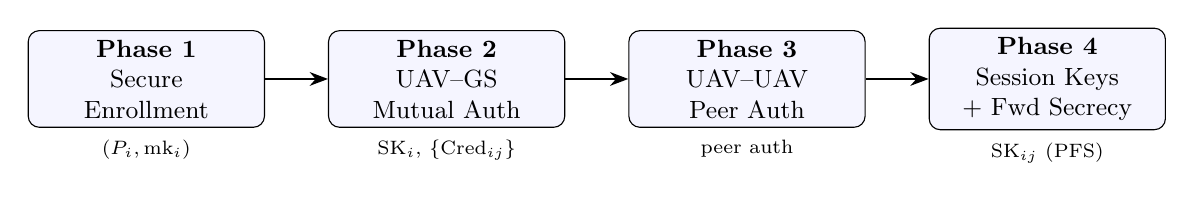
\begin{tikzpicture}[
  box/.style={draw,rounded corners,align=center,minimum height=1.15cm,
              minimum width=3.0cm,font=\small,fill=blue!4},
  >=Stealth]
\node[box] (p1) {\textbf{Phase 1}\\Secure\\Enrollment};
\node[box,right=0.8cm of p1] (p2) {\textbf{Phase 2}\\UAV--GS\\Mutual Auth};
\node[box,right=0.8cm of p2] (p3) {\textbf{Phase 3}\\UAV--UAV\\Peer Auth};
\node[box,right=0.8cm of p3] (p4) {\textbf{Phase 4}\\Session Keys\\+ Fwd Secrecy};
\draw[->,thick] (p1) -- (p2);
\draw[->,thick] (p2) -- (p3);
\draw[->,thick] (p3) -- (p4);
\node[font=\scriptsize,below=1pt of p1,align=center] {$(P_i,\text{mk}_i)$};
\node[font=\scriptsize,below=1pt of p2,align=center] {$\text{SK}_i$, $\{\text{Cred}_{ij}\}$};
\node[font=\scriptsize,below=1pt of p3,align=center] {peer auth};
\node[font=\scriptsize,below=1pt of p4,align=center] {$\text{SK}_{ij}$ (PFS)};
\end{tikzpicture}
\caption{The four phases and what each produces. Enrollment is performed once,
in a secure facility; Phases~2--4 run in the field.}
\label{fig:overview}
\end{figure}

\subsection{Phase~1: Secure Enrollment and Registration}
\label{subsec:phase1}

Enrollment runs once per UAV, in a physically secure facility over a trusted
channel (a wired link or a shielded RF cage), before the drone is deployed. Its
purpose is to establish the stable master key $\text{mk}_i$ and the public
helper data $P_i$, so that in the field the UAV can regenerate $\text{mk}_i$
from its own PUF without ever storing a secret.

\textbf{Step~1.1: PUF interrogation.}
The GS draws a block of $L$ random $128$-bit challenges
$\bm{C}_i=(C_i^{(1)},\dots,C_i^{(L)})$ and has the UAV evaluate its PUF on each:
\begin{equation}
R = \big(\,\text{PUF}_i(C_i^{(1)}),\ \dots,\ \text{PUF}_i(C_i^{(L)})\,\big).
\end{equation}
Concatenating $L$ blocks aggregates enough physical entropy to survive the
helper-data loss quantified below; $R$ is the raw enrollment response.

\textbf{Step~1.2: Key and helper-data generation.}
The GS runs the fuzzy-extractor generator $\mathsf{Gen}$ on $R$. It samples a
random seed, forms a code-offset sketch, and extracts the master key:
\begin{align}
c &= \mathsf{C}.\mathsf{Encode}(r), \quad r \xleftarrow{\$} \{0,1\}^{k}, &
s &= R \oplus c, \\[1ex]
\text{mk}_i &= \mathsf{KDF}\big(\mathsf{Ext}_{\text{seed}}(R);\ \texttt{root}\big), &
P_i &= (s,\ \text{seed}).
\end{align}
Here $s$ is the public sketch that will later let a noisy response be decoded
back to $R$, and $\mathsf{Ext}$ is a strong extractor (realised by the KDF) that
compresses $R$ into a near-uniform key. The pair $(P_i,\text{mk}_i)$ is the
output of $\mathsf{Gen}$.

\textbf{Step~1.3: Sizing the enrollment.}
Because the sketch $s$ leaks at most $n-k=124$ bits about each block
(Lemma~\ref{lem:helper}), the number of blocks $L$ is chosen so that the
entropy left after the leak still exceeds the desired key length $\ell$:
\begin{equation}
\sum_{b=1}^{L}\big(m_b-(n-k)\big)\ \ge\ \ell + 2\log(1/\varepsilon),
\label{eq:budget}
\end{equation}
where $m_b$ is the measured per-block min-entropy and $\varepsilon$ is a
negligible statistical-distance target. This inequality is what guarantees
$\text{mk}_i$ is a strong key rather than a slightly-random one.

\textbf{Step~1.4: Identity and pairwise-credential setup.}
The GS assigns a permanent identity and an initial rotating temporary identity,
and fixes a GS-only master key from which all per-pair credentials are derived:
\begin{align}
\text{TID}_i &= h(\text{ID}_i \,\|\, \text{seed}_i'), &
\text{Cred}_{ij} &= \mathsf{KDF}\big(\text{mk}_{\text{GS}};\ \texttt{pair\text{-}cred}\,\|\,\min(i,j)\,\|\,\max(i,j)\big).
\end{align}
The temporary identity hides the permanent one from eavesdroppers, and each
$\text{Cred}_{ij}$ is a distinct secret for exactly one pair. These credentials
are \emph{not} released here; they are delivered, encrypted, during Phase~2.

\textbf{Step~1.5: Storage.}
After enrollment:
\begin{itemize}[leftmargin=*]
  \item \textbf{GS stores} $\{\text{ID}_i,\ \text{TID}_i,\ \bm{C}_i,\ P_i,\ \text{mk}_i\}$ per UAV, plus the single master key $\text{mk}_{\text{GS}}$, all in tamper-resistant memory.
  \item \textbf{$\text{UAV}_i$ stores} $\{\text{TID}_i,\ \bm{C}_i,\ P_i\}$ only. Every one of these is public; \emph{no secret is stored on the drone}.
\end{itemize}
This is the central advantage of the design: capturing a UAV yields no key
material, because the master key exists only transiently, regenerated from the
PUF whenever it is needed.

\subsection{Phase~2: UAV--Ground Station Mutual Authentication}
\label{subsec:phase2}

Phase~2 runs when a UAV powers up in the field. It is a four-message exchange
that mutually authenticates the UAV and GS, establishes a forward-secret
session key $\text{SK}_i$, and delivers the UAV's per-pair credentials for
Phase~3. Both sides key their MACs with
$K^{i}_{\text{auth}}=\mathsf{KDF}(\text{mk}_i;\texttt{p2\text{-}auth})$: the GS
computes it from the stored $\text{mk}_i$, and the UAV regenerates
$\text{mk}_i$ from its PUF. Figure~\ref{fig:phase2} shows the message flow.

\begin{figure}[H]
\centering
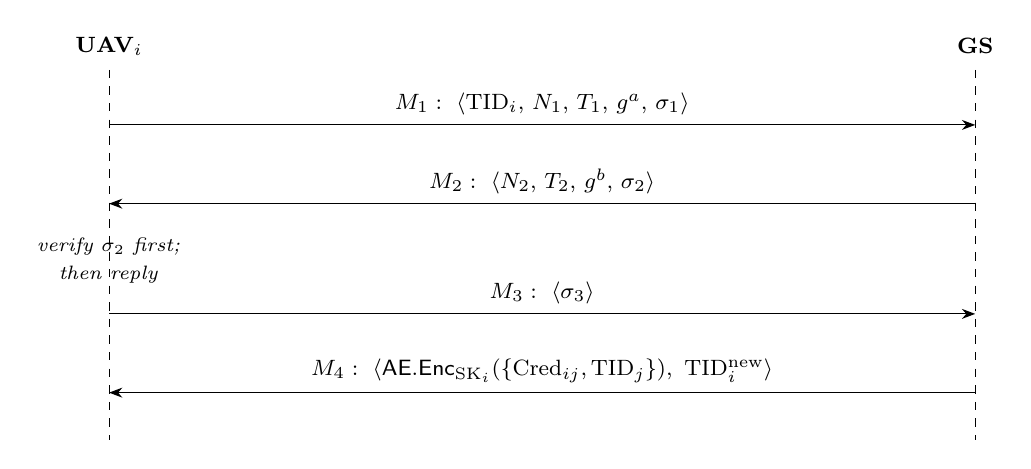
\begin{tikzpicture}[>=Stealth,font=\footnotesize]
  \node at (0,0) {\textbf{UAV$_i$}};
  \node at (11,0) {\textbf{GS}};
  \draw[dashed] (0,-0.3) -- (0,-5.0);
  \draw[dashed] (11,-0.3) -- (11,-5.0);
  \draw[->] (0,-1.0) -- node[above]{$M_1:\ \langle \text{TID}_i,\,N_1,\,T_1,\,g^{a},\,\sigma_1\rangle$} (11,-1.0);
  \draw[->] (11,-2.0) -- node[above]{$M_2:\ \langle N_2,\,T_2,\,g^{b},\,\sigma_2\rangle$} (0,-2.0);
  \node[align=left,font=\scriptsize] at (0,-2.55) {\emph{verify $\sigma_2$ first;}};
  \node[align=left,font=\scriptsize] at (0,-2.9) {\emph{then reply}};
  \draw[->] (0,-3.4) -- node[above]{$M_3:\ \langle \sigma_3\rangle$} (11,-3.4);
  \draw[->] (11,-4.4) -- node[above]{$M_4:\ \langle \mathsf{AE}.\mathsf{Enc}_{\text{SK}_i}(\{\text{Cred}_{ij},\text{TID}_j\}),\ \text{TID}_i^{\text{new}}\rangle$} (0,-4.4);
\end{tikzpicture}
\caption{Phase~2 message sequence. The UAV validates the GS's MAC before it
replies, so a fraudulent challenger receives no response; peer credentials are
delivered under authenticated encryption only after mutual authentication
succeeds.}
\label{fig:phase2}
\end{figure}

\textbf{Message~1 (Authentication request): $\text{UAV}_i \rightarrow \text{GS}$.}
The UAV picks a fresh nonce and an ephemeral Diffie--Hellman scalar, and
authenticates the opening message:
\begin{align}
N_1 &\xleftarrow{\$} \{0,1\}^{128}, \qquad a \xleftarrow{\$} \text{scalar}, \\[1ex]
\sigma_1 &= \mathsf{MAC}_{K^{i}_{\text{auth}}}\big(\texttt{M1}\,\|\,\text{TID}_i\,\|\,N_1\,\|\,T_1\,\|\,g^{a}\big), \\[1ex]
M_1 &= \langle \text{TID}_i,\ N_1,\ T_1,\ g^{a},\ \sigma_1 \rangle.
\end{align}
Because $\sigma_1$ is a MAC keyed by $K^{i}_{\text{auth}}$, only a party that
holds $\text{mk}_i$---that is, the genuine UAV (through its PUF) or the GS
(through its database)---can produce it. The tag $\texttt{M1}$ marks the
message type so that a message from one step can never be replayed as another.

\textbf{Message~2 (GS response): $\text{GS} \rightarrow \text{UAV}_i$.}
The GS checks the timestamp and the nonce for freshness, looks up
$\text{mk}_i$, verifies $\sigma_1$, and answers with its own nonce and
ephemeral share:
\begin{align}
N_2 &\xleftarrow{\$} \{0,1\}^{128}, \qquad b \xleftarrow{\$} \text{scalar}, \\[1ex]
\sigma_2 &= \mathsf{MAC}_{K^{i}_{\text{auth}}}\big(\texttt{M2}\,\|\,\text{TID}_i\,\|\,N_1\,\|\,N_2\,\|\,T_2\,\|\,g^{a}\,\|\,g^{b}\big), \\[1ex]
M_2 &= \langle N_2,\ T_2,\ g^{b},\ \sigma_2 \rangle.
\end{align}
The tag $\sigma_2$ authenticates the GS to the UAV: it binds both nonces and
both ephemeral shares under the shared key, so no network adversary can forge
or alter it.

\textbf{Message~3 (UAV confirmation): $\text{UAV}_i \rightarrow \text{GS}$.}
The UAV first regenerates its master key from its PUF and \emph{verifies
$\sigma_2$ before doing anything else}:
\begin{align}
\text{mk}_i &= \mathsf{Rep}\big(\text{PUF}_i(\bm{C}_i),\ P_i\big), \\[1ex]
&\text{abort silently if } \sigma_2 \text{ is invalid.}
\end{align}
This ``verify-before-respond'' rule is what prevents a fraudulent GS from using
the UAV as an oracle: an attacker who cannot forge $\sigma_2$ elicits no reply
at all. If the check passes, the UAV confirms the transcript:
\begin{align}
\sigma_3 &= \mathsf{MAC}_{K^{i}_{\text{auth}}}\big(\texttt{M3}\,\|\,\mathcal{T}\big), \qquad
M_3 = \langle \sigma_3 \rangle,
\end{align}
where the transcript $\mathcal{T}$ is the concatenation of all fields of $M_1$
and $M_2$. Note that the raw PUF response is consumed inside $\mathsf{Rep}$ and
\emph{never appears on the wire}; only a MAC over public values is sent.

\textbf{Message~4 (Confirmation and credential delivery): $\text{GS} \rightarrow \text{UAV}_i$.}
After verifying $\sigma_3$, both parties hold the same ingredients, so each
computes the forward-secret session key
\begin{equation}
\text{SK}_i = \mathsf{KDF}\big(\text{mk}_i \,\|\, g^{ab} \,\|\, \mathcal{T};\ \texttt{p2\text{-}sess}\big),
\label{eq:sk_p2}
\end{equation}
and the GS delivers the UAV's per-pair credentials and a fresh identity under
authenticated encryption keyed by $\text{SK}_i$:
\begin{align}
\text{CredPkg} &= \mathsf{AE}.\mathsf{Enc}_{\text{SK}_i}\big(\eta;\ \text{TID}_i;\ \{(\text{Cred}_{ij},\ \text{TID}_j)\}_{j\neq i}\big), \\[1ex]
\text{TID}_i^{\text{new}} &= h(\text{TID}_i \,\|\, \text{mk}_i \,\|\, N_1 \,\|\, N_2), \qquad
M_4 = \langle \text{CredPkg},\ \text{TID}_i^{\text{new}} \rangle.
\end{align}
Authenticated encryption gives the credentials both confidentiality and
integrity: an eavesdropper learns nothing about any $\text{Cred}_{ij}$, and a
tampered package is rejected. The session key mixes in the Diffie--Hellman
secret $g^{ab}$, which is what makes it forward-secret (Phase~4). After
Phase~2 the UAV holds $\text{SK}_i$, its peer credentials
$\{\text{Cred}_{ij}\}$, and a rotated identity.

\subsection{Phase~3: UAV-to-UAV Peer Authentication}
\label{subsec:phase3}

Phase~3 lets any two UAVs authenticate each other directly, using the per-pair
credential $\text{Cred}_{ij}$ that each received (encrypted) in Phase~2. It
needs no GS involvement, so it works even when the GS link is down. Both sides
key their MACs with
$K^{ij}_{\text{auth}}=\mathsf{KDF}(\text{Cred}_{ij};\texttt{peer\text{-}auth})$.
Figure~\ref{fig:phase3} shows the three-message flow.

\begin{figure}[H]
\centering
\begin{tikzpicture}[>=Stealth,font=\footnotesize]
  \node at (0,0) {\textbf{UAV$_i$}};
  \node at (11,0) {\textbf{UAV$_j$}};
  \draw[dashed] (0,-0.3) -- (0,-4.0);
  \draw[dashed] (11,-0.3) -- (11,-4.0);
  \draw[->] (0,-1.0) -- node[above]{$P_1:\ \langle n_i,\,T,\,g^{a'},\,\tau_1\rangle$} (11,-1.0);
  \draw[->] (11,-2.2) -- node[above]{$P_2:\ \langle n_j,\,g^{b'},\,\tau_2\rangle$} (0,-2.2);
  \draw[->] (0,-3.4) -- node[above]{$P_3:\ \langle \tau_3\rangle$} (11,-3.4);
\end{tikzpicture}
\caption{Phase~3 message sequence. Every token is a MAC keyed by the per-pair
credential $\text{Cred}_{ij}$ and tagged with its message type, so tokens
cannot be reflected or reused across steps.}
\label{fig:phase3}
\end{figure}

\textbf{Message~P1 (Peer request): $\text{UAV}_i \rightarrow \text{UAV}_j$.}
The initiator picks a fresh nonce and ephemeral share and sends an
authenticated request:
\begin{align}
n_i &\xleftarrow{\$} \{0,1\}^{128}, \qquad a' \xleftarrow{\$} \text{scalar}, \\[1ex]
\tau_1 &= \mathsf{MAC}_{K^{ij}_{\text{auth}}}\big(\texttt{P1}\,\|\,i\,\|\,j\,\|\,n_i\,\|\,T\,\|\,g^{a'}\big), \qquad
P_1 = \langle n_i,\ T,\ g^{a'},\ \tau_1 \rangle.
\end{align}
Because $\tau_1$ is keyed by $\text{Cred}_{ij}$, which only $\text{UAV}_i$ and
$\text{UAV}_j$ possess, a third party---even one holding some other pair's
credential---cannot produce it.

\textbf{Message~P2 (Peer response): $\text{UAV}_j \rightarrow \text{UAV}_i$.}
The responder verifies $\tau_1$, then answers with its own nonce and share:
\begin{align}
\tau_2 &= \mathsf{MAC}_{K^{ij}_{\text{auth}}}\big(\texttt{P2}\,\|\,i\,\|\,j\,\|\,n_i\,\|\,n_j\,\|\,g^{a'}\,\|\,g^{b'}\big), \qquad
P_2 = \langle n_j,\ g^{b'},\ \tau_2 \rangle.
\end{align}
$\tau_2$ binds both identities and both nonces, so it authenticates
$\text{UAV}_j$ to $\text{UAV}_i$ and confirms that both are in the same fresh
session.

\textbf{Message~P3 (Completion): $\text{UAV}_i \rightarrow \text{UAV}_j$.}
The initiator verifies $\tau_2$ and closes the handshake with a final tag over
the transcript $\mathcal{T}=P_1\|P_2$:
\begin{align}
\tau_3 &= \mathsf{MAC}_{K^{ij}_{\text{auth}}}\big(\texttt{P3}\,\|\,\mathcal{T}\big), \qquad
P_3 = \langle \tau_3 \rangle.
\end{align}
The three distinct type tags ($\texttt{P1},\texttt{P2},\texttt{P3}$) ensure a
token from one step can never be replayed as another, which rules out
reflection attacks. For a swarm of $N$ UAVs, full-mesh peer authentication runs
$N(N-1)/2$ independent Phase~3 exchanges (for example, $45$ for $N=10$), all of
which may proceed in parallel.

\subsection{Phase~4: Session Key Establishment and Forward Secrecy}
\label{subsec:phase4}

Phase~4 is the keying that both interactive phases finish with. In Phase~2 the
UAV--GS key is $\text{SK}_i$ of Eq.~\eqref{eq:sk_p2}; in Phase~3 the peer key is
\begin{equation}
\text{SK}_{ij} = \mathsf{KDF}\big(\text{Cred}_{ij}\,\|\,g^{a'b'}\,\|\,\mathcal{T};\ \texttt{peer\text{-}sess}\big).
\label{eq:sk_p3}
\end{equation}
Both keys have the same shape, which we write uniformly as
\begin{equation}
\text{SK} = \mathsf{KDF}\big(\underbrace{k_{\text{lt}}}_{\text{mk}_i\ \text{or}\ \text{Cred}_{ij}} \,\|\, g^{xy} \,\|\, \mathcal{T};\ \ell\big).
\label{eq:sk_unified}
\end{equation}
Two independent secrets go into every session key. The first is the long-term
key $k_{\text{lt}}$, which ties the session to the PUF (via $\text{mk}_i$) or to
the pair (via $\text{Cred}_{ij}$). The second is the ephemeral Diffie--Hellman
secret $g^{xy}$, whose public shares were authenticated inside the MAC
transcript of the corresponding handshake. Mixing in $g^{xy}$ is what provides
\emph{perfect forward secrecy}: once the ephemeral scalars are erased, an
adversary who later learns $k_{\text{lt}}$ still cannot reconstruct a past key,
because doing so would require solving Diffie--Hellman on the recorded shares.
The exchange is mandatory---there is no derivation path that omits $g^{xy}$---so
a session either establishes a forward-secret key or fails.

% ══════════════════════════════════════════════════════════════
% SECTION 5: SECURITY ANALYSIS
% ══════════════════════════════════════════════════════════════
\section{Security Analysis}
\label{sec:security}

We now analyse the protocol formally. Each theorem is proved by reducing an
attack to the violation of a standard assumption; the reductions are then
mirrored by a symbolic model (\S\ref{subsec:symbolic}).

\subsection{Assumptions}
\label{subsec:assumptions}

The proofs rely on the following standard assumptions.
\begin{enumerate}[leftmargin=*]
  \item \textbf{Hash security.} $h$ is pre-image, second-pre-image, and
  collision resistant; in the reductions it is modelled as a random oracle.
  \item \textbf{MAC unforgeability.} $\mathsf{MAC}$ is existentially unforgeable
  under chosen-message attack (EUF-CMA): without the key, a fresh valid tag can
  be produced only with negligible probability.
  \item \textbf{AEAD security.} $\mathsf{AE}$ provides ciphertext
  indistinguishability (IND-CCA) and ciphertext integrity (INT-CTXT).
  \item \textbf{PUF unpredictability.} Given polynomially many
  challenge--response pairs, the response to a fresh challenge is
  computationally indistinguishable from uniform to an adversary that does not
  possess the device; invasive probing destroys the PUF.
  \item \textbf{Diffie--Hellman.} The gap computational Diffie--Hellman
  (gap-CDH) problem is hard in $\mathbb{G}$.
\end{enumerate}

We first record the helper-data property that underpins the strength of the
master key.

\begin{lemma}[Helper-data privacy]
\label{lem:helper}
Let the enrollment response $R$ have conditional min-entropy $\widetilde{H}_\infty(R)=m$.
The code-offset sketch $s=R\oplus c$ discloses at most $n-k$ bits, so
\begin{equation}
\widetilde{H}_\infty\big(R \mid P\big)\ \ge\ m-(n-k).
\end{equation}
Consequently, if the extractor output length $\ell$ satisfies
$\ell \le m-(n-k)-2\log(1/\varepsilon)$, then $\text{mk}$ is within statistical
distance $\varepsilon$ of uniform given the public helper data $P$.
\end{lemma}

\begin{proof}
Given the internal randomness $r$, the sketch $s=R\oplus c$ is a deterministic
function of $R$ that pins $R$ to a coset of the $[n,k]$ code $\mathsf{C}$;
revealing that coset fixes at most $n-k$ syndrome bits, so by the chain rule for
average min-entropy $\widetilde{H}_\infty(R\mid s)\ge \widetilde{H}_\infty(R)-(n-k)$, and the seed is
independent of $R$. Applying the strong-extractor property to the residual
source gives a key within distance $\varepsilon$ of uniform. \qed
\end{proof}

\subsection{Phase~2: Mutual Authentication}

\begin{theorem}[Phase~2 mutual authentication]
\label{thm:mutual_auth}
After a successful Phase~2 exchange, $\text{UAV}_i$ and the GS have mutually
authenticated one another, and both agree on the transcript $\mathcal{T}$,
except with negligible probability.
\end{theorem}

\begin{proof}
Both directions rest on the MAC key $K^{i}_{\text{auth}}=\mathsf{KDF}(\text{mk}_i;\texttt{p2\text{-}auth})$,
which by Lemma~\ref{lem:helper} and PUF unpredictability is unknown to any
adversary lacking either the PUF or the GS database.
\emph{(GS authenticates UAV.)} The GS accepts only if $\sigma_1$ (and later
$\sigma_3$) verifies under $K^{i}_{\text{auth}}$; producing a fresh valid tag
without the key is exactly an EUF-CMA forgery.
\emph{(UAV authenticates GS.)} Symmetrically, the UAV accepts only if $\sigma_2$
verifies; although every field inside $\sigma_2$ is public, the \emph{key} is
secret, so a fresh valid $\sigma_2$ is again a forgery.
A nonce collision that could enable transcript reuse occurs with probability at
most $q^2/2^{128}$ for $q$ sessions. Absent forgery and collision, the two
accepting parties share identical fields in $M_1$ and $M_2$, i.e.\ they agree on
$\mathcal{T}$. \qed
\end{proof}

\begin{corollary}[No PUF read-out oracle]
\label{cor:oracle}
An adversary that impersonates the GS learns no PUF response, so it cannot
harvest challenge--response pairs to model the PUF.
\end{corollary}

\begin{proof}
By the verify-before-respond rule, the UAV emits $M_3$ only after $\sigma_2$
verifies, which by Theorem~\ref{thm:mutual_auth} an adversary can force only by
forging a MAC. When the check fails the UAV sends nothing; when it passes, the
only value on the wire is $\sigma_3$, a MAC over public transcript fields---the
PUF response is consumed inside $\mathsf{Rep}$ and is never transmitted. Hence
no challenge--response pair is exposed. \qed
\end{proof}

\subsection{Replay Attack Resistance}

\begin{theorem}[Replay resistance]
\label{thm:replay}
Phase~2 and Phase~3 resist replay attacks.
\end{theorem}

\begin{proof}
Three mechanisms combine. First, every message carries a fresh $128$-bit nonce
and a timestamp verified within a window $\Delta T$; a verbatim replay reuses a
stale nonce or timestamp and is rejected. Second, each MAC binds a per-message
type tag ($\texttt{M1},\dots,\texttt{P3}$), so a token from one step cannot be
accepted at another. Third, from the second message onward each MAC binds the
partner's nonce, so a token from one session cannot be reused in another without
producing a mismatch---which, by Theorems~\ref{thm:mutual_auth}
and~\ref{thm:peer_auth}, would require a forgery. \qed
\end{proof}

\subsection{Phase~3: Peer Mutual Authentication}

\begin{theorem}[Peer mutual authentication]
\label{thm:peer_auth}
After a successful Phase~3 exchange, $\text{UAV}_i$ and $\text{UAV}_j$ have
mutually authenticated one another, without GS involvement, and no per-pair
secret is exposed in transit.
\end{theorem}

\begin{proof}
The credential $\text{Cred}_{ij}$ reaches each endpoint only inside the Phase~2
package $\mathsf{AE}.\mathsf{Enc}_{\text{SK}_i}(\cdots)$; by INT-CTXT the
adversary cannot make a UAV accept a substituted credential, and by IND-CCA it
learns nothing about $\text{Cred}_{ij}$. Given a secret $\text{Cred}_{ij}$, the
tokens $\tau_1,\tau_2,\tau_3$ are MACs under
$K^{ij}_{\text{auth}}$; each binds both identities and both nonces, so a fresh
acceptance forces a matching computation by the partner---otherwise an EUF-CMA
forgery. Because credentials are pair-specific, a third party holding some other
$\text{Cred}_{k\ell}$ has no information about $\text{Cred}_{ij}$ and cannot
assert identity $i$ to $j$. \qed
\end{proof}

\subsection{Man-in-the-Middle Resistance}

\begin{theorem}[MITM resistance]
\label{thm:mitm}
The protocol resists active man-in-the-middle attacks in both Phase~2 and
Phase~3.
\end{theorem}

\begin{proof}
Every accepted message is a MAC (or an authenticated ciphertext) over a
transcript that includes fresh nonces, a timestamp, a type tag, and---from the
second message onward---the partner's nonce and ephemeral share. Altering any
field invalidates the covering tag, and forging a new tag requires the secret
key (EUF-CMA / INT-CTXT). By the agreement guarantees of
Theorems~\ref{thm:mutual_auth} and~\ref{thm:peer_auth}, both endpoints therefore
hold the identical transcript, so an interposed adversary cannot sit undetected
between them. \qed
\end{proof}

\subsection{Session-Key Secrecy and Forward Secrecy}

\begin{theorem}[Session-key secrecy]
\label{thm:key_secrecy}
For an adversary that corrupts neither endpoint of the target session, the
session key of Eq.~\eqref{eq:sk_unified} is indistinguishable from uniform.
\end{theorem}

\begin{proof}
The key is $\mathsf{KDF}(k_{\text{lt}}\|g^{xy}\|\mathcal{T})$. Two independent
secrets protect it: the long-term key $k_{\text{lt}}$
($\text{mk}_i$ by Lemma~\ref{lem:helper} and PUF unpredictability, or
$\text{Cred}_{ij}$ by IND-CCA of its delivery, Theorem~\ref{thm:peer_auth}) and
the Diffie--Hellman secret $g^{xy}$. Modelling the KDF as a pseudorandom
function, replacing it by a random function is undetectable up to its PRF
advantage; the input $g^{xy}$ is unpredictable under gap-CDH given only the
authenticated shares $g^{x},g^{y}$. Hence the output is uniform up to negligible
terms. \qed
\end{proof}

\begin{theorem}[Perfect forward secrecy]
\label{thm:pfs}
If the ephemeral scalars are erased after use, then revealing the long-term
secrets ($\text{mk}_i$, $\text{Cred}_{ij}$, or $\text{mk}_{\text{GS}}$)
\emph{after} a target session closes does not compromise that session's key.
\end{theorem}

\begin{proof}
A post-session reveal gives the adversary $k_{\text{lt}}$ but not the erased
scalars $x,y$. The key of Eq.~\eqref{eq:sk_unified} still depends on $g^{xy}$,
which the adversary must now compute from the recorded, authenticated shares
$g^{x},g^{y}$---a gap-CDH instance. Because the ephemeral exchange is mandatory,
there is no non-ephemeral key to fall back on. Hence past keys remain
indistinguishable from uniform. \qed
\end{proof}

\subsection{Physical Capture Resistance}

\begin{theorem}[Physical capture resistance]
\label{thm:capture}
Capturing $\text{UAV}_k$ and reading its NVM does not let the adversary
impersonate any other UAV to the GS, nor impersonate any peer pair that does not
involve $k$. A captured node's peer exposure is limited to its own $N-1$ links.
\end{theorem}

\begin{proof}
The NVM of $\text{UAV}_k$ holds only $\{\text{TID}_k,\ \bm{C}_k,\ P_k,\ \{\text{Cred}_{kj}\}_j\}$
plus any live session keys; all of $\text{TID}_k,\bm{C}_k,P_k$ are public.
Impersonating $\text{UAV}_m$ ($m\neq k$) in a fresh Phase~2 needs
$K^{m}_{\text{auth}}=\mathsf{KDF}(\text{mk}_m;\cdot)$; but $\text{mk}_m$ is never
stored, is not recoverable from $k$'s silicon (tamper evidence), and is
unpredictable (PUF assumption), so this reduces to a MAC forgery. Impersonating
a pair $(m,\ell)$ with $k\notin\{m,\ell\}$ needs
$\text{Cred}_{m\ell}=\mathsf{KDF}(\text{mk}_{\text{GS}};\cdot)$, which is
independent of every captured $\text{Cred}_{kj}$ (distinct KDF inputs, and
$\text{mk}_{\text{GS}}$ never leaves the GS). Only pairs that include $k$ share a
captured credential, giving the stated $N-1$ exposure. \qed
\end{proof}

\subsection{Symbolic Verification}
\label{subsec:symbolic}

The computational theorems are corroborated by a symbolic model in the Tamarin
prover~\cite{tamarin}, whose multiset-rewriting calculus expresses freshness,
stateful credential issuance, and device-compromise events natively. In the
model, $h,\mathsf{MAC},\mathsf{AE},\mathsf{KDF}$ are function symbols with the
usual equational theory, each PUF is a private per-device function, and helper
data and all wire terms are public. The Dolev--Yao adversary controls the
network; two extra rules model compromise---one that reveals a captured node's
NVM (its identities, helper data, and per-pair credentials, but neither its PUF
nor its master key) and one that reveals long-term secrets after a session
closes, for the forward-secrecy query. The prover discharges lemmas that
correspond one-to-one with the theorems above: injective agreement for Phase~2
and Phase~3 (Theorems~\ref{thm:mutual_auth} and~\ref{thm:peer_auth}), a
no-replay lemma (Theorem~\ref{thm:replay}), a capture-isolation lemma
(Theorem~\ref{thm:capture}), a session-key-secrecy lemma
(Theorem~\ref{thm:key_secrecy}), and a forward-secrecy lemma
(Theorem~\ref{thm:pfs}). The PUF's noise is idealised as a noiseless private
function---its error tolerance is the computational correctness property of the
fuzzy extractor---and confidential delivery is abstracted by a symmetric
encryption operator, leaving the fine-grained secrecy argument to the
computational analysis.

\subsection{Summary of Security Properties}

Table~\ref{tab:security_summary} summarises the guarantees and the mechanism
behind each.

\begin{table}[H]
\centering
\caption{Summary of Security Properties}
\label{tab:security_summary}
\begin{tabular}{@{}p{4.6cm}cp{6.0cm}@{}}
\toprule
\textbf{Property} & \textbf{Result} & \textbf{Mechanism} \\
\midrule
UAV--GS mutual auth & Thm~\ref{thm:mutual_auth} & Keyed MAC under PUF-derived $\text{mk}_i$ \\
No PUF read-out oracle & Cor~\ref{cor:oracle} & Verify-before-respond; response stays on-device \\
Replay resistance & Thm~\ref{thm:replay} & Nonces + timestamps + type tags \\
Peer mutual auth & Thm~\ref{thm:peer_auth} & Per-pair credential + keyed MAC \\
MITM resistance & Thm~\ref{thm:mitm} & Transcript-binding MACs / AEAD \\
Session-key secrecy & Thm~\ref{thm:key_secrecy} & KDF over long-term key and DH secret \\
Perfect forward secrecy & Thm~\ref{thm:pfs} & Mandatory authenticated ephemeral DH \\
Physical-capture resistance & Thm~\ref{thm:capture} & No stored key; per-pair credentials \\
Identity anonymity & --- & Rotating temporary identities \\
\bottomrule
\end{tabular}
\end{table}

% ══════════════════════════════════════════════════════════════
% SECTION: REFERENCE IMPLEMENTATION
% ══════════════════════════════════════════════════════════════
\section{Reference Implementation}
\label{sec:implementation}

The protocol of Section~\ref{sec:protocol} is implemented in C++17 on
OMNeT++~6.3. This section records the concrete primitive choices, the
parameterisation of the fuzzy extractor, and the verification evidence for each
component, so that every number in Section~\ref{sec:results} can be traced to a
specific mechanism.

\subsection{Structure}

The implementation separates protocol logic from simulation machinery. The classes
implementing Phases~1--4 depend only on abstract cryptographic interfaces and on
byte strings; they contain no reference to the simulation kernel. This allows the
entire four-phase exchange to be driven over an in-memory transport and validated
independently of the network model, which is how the protocol-level results in
Section~\ref{subsec:functional} were obtained.

A single transmission module owns the link-delay model, so propagation,
serialisation, processing delay, and jitter are defined once rather than
duplicated per node type. The same module provides the interception point used by
the adversary of Section~\ref{subsec:security_eval}; when no adversary is present
it forwards immediately, so attack and baseline runs remain directly comparable.

\subsection{Canonical message encoding}

Every message is serialised by one encoder, whose output serves simultaneously as
the wire image, the input to the message-authentication code, and the byte count
driving the link delay. Each field is emitted as a type tag, a two-byte length,
and its value, under a header carrying the protocol version, the suite identifier,
and a per-message-type tag:
%
\begin{align}
\mathsf{field}(t,v) &= \mathsf{u8}(t)\,\|\,\mathsf{u16}(|v|)\,\|\,v,\\[0.5ex]
\mathsf{enc} &= \mathsf{u8}(\mathrm{ver})\,\|\,\mathsf{u8}(\mathrm{suite})\,\|\,
                \mathsf{u8}(\mathrm{type})\,\|\,\mathsf{u16}(k)\,\|\,
                \mathsf{field}(t_1,v_1)\cdots
\end{align}
%
with tags emitted in strictly ascending order. The encoding is therefore
\emph{injective} (no two distinct field sets share a byte string) and
\emph{canonical} (each field set has exactly one valid encoding), which is the
precondition the unforgeability argument of Section~\ref{sec:security} requires of
its MAC inputs. Because the same encoder produces the transmitted bytes, reported
communication overhead cannot drift from what is actually sent. Non-canonical
input --- duplicate or out-of-order tags --- is rejected rather than accepted, and
reading an absent field raises an error instead of yielding an empty buffer.

\subsection{Cryptographic suites}

Two interoperable suites implement the same abstract interface, selected by one
parameter. Table~\ref{tab:suites} lists them.

\begin{table}[H]
\centering
\caption{The two cryptographic profiles}
\label{tab:suites}
\small
\begin{tabular}{@{}p{2.9cm}p{4.6cm}p{4.6cm}@{}}
\toprule
\textbf{Component} & \textbf{Profile \texttt{sha3}} & \textbf{Profile \texttt{spongent}} \\
\midrule
Hash $h(\cdot)$ & SHA3-256 truncated to 160 bits & SPONGENT-160/160/16 \\
MAC & HMAC-SHA3-256, 128-bit tag & prefix keyed sponge, 128-bit tag \\
KDF & HKDF (extract-then-expand) & one-pass sponge \\
AEAD & ChaCha20-Poly1305 & Ascon-128a v1.2 \\
Key exchange & X25519 & X25519 \\
Hash/MAC level & 128-bit & 80-bit ($c=160$) \\
Provenance & OpenSSL~3.5 & vendored \\
\bottomrule
\end{tabular}
\end{table}

Three points require explicit statement.

\textbf{HMAC is not applicable to the sponge profile.} HMAC is defined over a
compression function of block size $B$ and requires $|K|\le B$. For
SPONGENT-160/160/16 the rate is $16$~bits, so the block is two bytes --- smaller
than any useful key --- and hashing the key first still exceeds it. The
construction is therefore undefined, and any ad-hoc substitution would have no
supporting proof. The sponge profile instead uses the standard prefix keyed sponge
underlying KMAC~\cite{sha3_standard}, which is sound for a sponge and does not
require HMAC's nested structure: a sponge with non-zero capacity is not
length-extendable, so the nesting HMAC exists to provide is unnecessary.

\textbf{The sponge profile operates at the 80-bit level.} With capacity $c=160$
the keyed-sponge bound gives approximately $c/2 = 80$~bits, matching the
collision resistance of a 160-bit digest but deliberately asymmetric with the
128-bit AEAD and key-exchange components. It is presented as a constrained-hardware
profile at that level rather than as a 128-bit one.

\textbf{Key derivation is domain-separated.} Distinct leading bytes separate the
hash, MAC, and KDF modes even where they share a permutation, and every derived
key carries a unique label (\texttt{p2-auth}, \texttt{p2-sess}, \texttt{pair-cred},
\texttt{peer-auth}, \texttt{peer-sess}, \texttt{tid-rotate}), so a key minted for
one purpose cannot be mistaken for another.

All protocol randomness --- nonces, ephemeral scalars, extractor seeds, enrollment
challenges --- is drawn from a deterministic generator seeded from the simulator's
random-number stream. Ephemeral X25519 keys are loaded from those bytes rather
than generated internally by the library, so an entire run, including every
ephemeral key, is reproducible from its configured seed.

\subsection{Error-correcting code}

The generator polynomial is formed as the product of the minimal polynomials of
$\alpha^1,\dots,\alpha^{2t}$ over the \emph{complete} conjugate closure of each
root. For $t=18$ over $\mathrm{GF}(2^8)$ the closure contains $124$ roots, giving
$\deg g = 124$ with binary coefficients and therefore
%
\begin{equation}
\mathrm{BCH}(n{=}255,\ k{=}131,\ t{=}18), \qquad n-k = 124 \ \text{parity bits}.
\end{equation}
%
Both properties are asserted at construction: a non-binary coefficient indicates
an incomplete closure, and the parity length is computed rather than assumed. This
matters because $k = 131 \ge 128$ is what allows a full response block to be
protected; taking the parity length as $mt = 144$ instead would give $k = 111$ and
silently leave the tail of every response uncovered.

Decoding proceeds by syndrome computation, the Berlekamp--Massey algorithm, and a
Chien search, followed by a verification that the corrected word has all-zero
syndromes. Failure is reported as failure: the decoder never returns the
uncorrected input while indicating success.

\subsection{Fuzzy-extractor parameterisation}

Enrollment applies $\mathsf{Gen}$ to a response of $L$ blocks of $n=255$ bits;
reproduction applies $\mathsf{Rep}$ with the public helper data. Two consequences
of Lemma~\ref{lem:helper} drive the parameter choice.

First, since the sketch discloses up to $n-k$ bits per block, the block length
must exceed the leak by a useful margin. A $128$-bit block against a $124$-bit
leak contributes almost nothing, which is why blocks are $255$ bits --- matching
the code length. A construction that sized blocks to the native response width of
a $128$-bit challenge--response pair could not satisfy Eq.~\eqref{eq:budget_impl}
at any block count.
Second, the budget
%
\begin{equation}
L\left(\rho n - (n-k)\right) \;\ge\; \ell + 2\log_2(1/\varepsilon)
\label{eq:budget_impl}
\end{equation}
%
is enforced at construction and raises an error when unmet, rather than being
documented and left to the caller. With $\rho = 0.95$, $\ell = 256$ and
$\varepsilon = 2^{-64}$, each block contributes $118.25$ bits and $L=4$ gives
$473 \ge 384$.

Three profiles are provided (Table~\ref{tab:fe_profiles}). The default uses the
parameters of Section~\ref{sec:protocol}; the third concatenates a $[3,1,3]$
repetition inner code, which must operate on repeated measurements of the same
physical bit. Enrollment fixes a reference and publishes each copy's offset as
additional helper data; reproduction removes those offsets before voting, reducing
the per-bit error rate from $p$ to approximately $3p^2$. The inner offsets are
charged to the leak accounting at $(\mathrm{rep}-1)$ bits per outer bit.

\begin{table}[H]
\centering
\caption{Fuzzy-extractor profiles}
\label{tab:fe_profiles}
\small
\begin{tabular}{@{}lcccc@{}}
\toprule
\textbf{Profile} & \textbf{Code} & \textbf{$L$} & \textbf{PUF bits} & \textbf{Leak (bits)} \\
\midrule
\texttt{bch255-131-18} (default) & BCH(255,131,18) & 4 & 1020 & 496 \\
\texttt{bch255-91-25} & BCH(255,91,25) & 5 & 1275 & 820 \\
\texttt{rep3-bch255-131-18} & $[3,1,3]\oplus$BCH(255,131,18) & 5 & 3825 & 3170 \\
\bottomrule
\end{tabular}
\end{table}

Reproduction fails closed. If any block fails to decode, no key material is
returned: a partially recovered response is never converted into a key.

\subsection{PUF models}

Three models are provided, and results state which one they rest on. An
\emph{idealised} model realises the strong-PUF abstraction as a keyed
pseudorandom function and is used where near-uniform responses are the intended
assumption. An \emph{arbiter} model implements the additive-delay formulation over
128 stages with per-device Gaussian delay weights. A third XORs $k$ arbiter chains.

Both models produce a whole response from one keyed stream rather than one
evaluation per bit. The idealised model returns
%
\begin{equation}
R = \mathsf{HMAC}_{\text{SHA3-256}}\big(k_{\text{dev}},\ \ell \,\|\, C \,\|\, n\big)_{n \ge 0}
    \ \big|_{\le b\ \text{bits}},
\label{eq:puf_stream}
\end{equation}
%
the concatenation of successive 256-bit blocks, truncated to the response length
$b$; four calls cover the $1020$-bit response the default profile requires. The
arbiter model takes all of its per-bit sub-challenges from one
$\mathsf{SHA3\text{-}256}$ stream over $(\ell,|C|,C,n)$ in the same way. This is a
simulation-cost decision with no cryptographic consequence: the object is the same
keyed PRF per device with independent uniform output bits, whereas evaluating each
bit separately cost two hash calls per bit and made the simulated PUF the slowest
component of a protocol whose real device answers in nanoseconds.

Response noise is applied as a 16-bit threshold on two DRBG bytes per bit,
\begin{equation}
\text{flip}_j = \big[\ \mathsf{u16}(z_{2j}, z_{2j+1}) < \lfloor p \cdot 2^{16} \rfloor\ \big],
\end{equation}
which is an exact Bernoulli$(p)$ channel to $16$-bit precision and costs a
fraction of a per-bit floating-point draw. Two bytes are drawn per bit whatever
$p$ is, so the generator's stream position after an evaluation does not depend on
the noise setting and a run stays reproducible when that setting changes.

In the arbiter model, measurement noise is added to the accumulated \emph{delay
difference} rather than by flipping output bits:
%
\begin{equation}
\Delta' = \sum_{i} w_i \phi_i + \mathcal{N}(0,\sigma), \qquad
r = \mathbb{1}[\Delta' > 0].
\end{equation}
%
Bits whose delay difference lies near zero therefore flip far more often than the
rest, reproducing the reliability profile of real silicon. The measured variance of
per-bit flip rates is approximately $98\times$ that of a uniform bit-flip channel,
a structural property a per-bit model cannot exhibit. A calibration routine
converts a target average bit-error rate into the corresponding $\sigma$.

Measured characteristics over 24 devices and 276 device pairs: inter-device Hamming
distance $0.5019$ for the arbiter model and $0.5026$ for the idealised model, both
consistent with the ideal $0.5$; calibrated bit-error rates track their targets to
within $0.2$ percentage points across $1\%$--$10\%$.

\subsection{Verification of primitives}

Each primitive is checked against published reference values where they exist, and
reports its verification status programmatically. Table~\ref{tab:kat} summarises.

\begin{table}[H]
\centering
\caption{Verification evidence per primitive}
\label{tab:kat}
\small
\begin{tabular}{@{}p{3.4cm}p{8.4cm}@{}}
\toprule
\textbf{Primitive} & \textbf{Evidence} \\
\midrule
SHA3-256 & FIPS~202 / CAVP short-message vectors \\
HMAC-SHA3-256 & NIST example values with intermediate results \\
HKDF & RFC~5869, Appendices A.1--A.3 \\
ChaCha20-Poly1305 & RFC~8439, Section~2.8.2 \\
X25519 & RFC~7748, Section~6.1; low-order points rejected \\
Ascon-128a & all 1089 vectors of the official LWC known-answer-test file \\
SPONGENT-160 & byte-exact against the designers' reference implementation and the
published \texttt{"Sponge + Present = Spongent"} digest; no official
known-answer-test file exists for SPONGENT, and none is claimed \\
BCH(255,131,18) & $\deg g = 124$; $g(x) \mid x^{255}+1$; exact recovery in all
18{,}000 trials across weights $1$--$18$; failure correctly reported beyond the
radius in 3{,}000 trials \\
\bottomrule
\end{tabular}
\end{table}

Neither vendored primitive has undergone timing or side-channel analysis; tag
comparisons use a constant-time routine and no branch depends on secret data, but
nothing stronger is claimed. The verification-status strings state this, and a
regression test fails if the qualification is removed.

The complete unit suite comprises twelve test programs and approximately
$4.5\times10^{5}$ assertions, covering the primitives above, the encoding, the
fuzzy extractor, the PUF models, the wire round-trip, the signature baselines, and
the full four-phase exchange.

\subsection{Simulation model}
\label{subsec:simmodel}

The scenario places $N$ UAVs around a $500\times300$~m field with the ground
station at its centre. Link delay is the sum of propagation (from node
coordinates), serialisation at the configured bit rate, a fixed processing delay,
and half-normal jitter, each reported separately per message. This primary model
does not itself simulate MAC-layer contention, so its reported network delay is a
lower bound; \S\ref{subsec:inet} reports a second, independent measurement of the
same Phase-2 handshake over a real IEEE~802.11 stack with genuine CSMA/CA
contention, so that lower bound is now bracketed by an upper one rather than left
undisclosed.

All node parameters are declared with defaults and are therefore overridable from
the configuration file, and statistics are declared so that both scalar and vector
outputs are recorded.

\subsection{Evaluation scenarios}
\label{subsec:scenarios}

Every scenario in Section~\ref{sec:results} changes exactly one variable relative
to the reference configuration \texttt{StadiumSHA3} and holds everything else
fixed, so that a difference in outcome can be attributed to that one variable
rather than to a confound. Table~\ref{tab:scenarios} lists all sixteen
configurations, the single variable each isolates, and which table or figure
reports its result, so the purpose of every run in the evaluation is stated in
one place rather than left implicit.

\begin{table}[H]
\centering
\caption{Every evaluation scenario, the variable it isolates, and where its
result is reported}
\label{tab:scenarios}
\footnotesize
\begin{tabular}{@{}p{3.1cm}p{4.2cm}p{5.4cm}p{1.6cm}@{}}
\toprule
\textbf{Scenario} & \textbf{Variable isolated} & \textbf{Question it answers} & \textbf{Reported in} \\
\midrule
\texttt{StadiumSHA3} & reference point: $N{=}10$, software-oriented suite & What does the protocol cost under its default, intended deployment? & Tab.~\ref{tab:functional}--\ref{tab:latency} \\
\texttt{StadiumSPONGENT} & crypto suite (\texttt{sha3} $\rightarrow$ \texttt{spongent}), $N$ unchanged & Does swapping to the hardware-oriented suite change correctness, and by how much does it change cost? & Tab.~\ref{tab:functional}--\ref{tab:latency} \\
\texttt{Baseline5UAV} & swarm size, $N{=}5$ & Lower end of the scaling curve & Tab.~\ref{tab:functional}--\ref{tab:latency} \\
\texttt{Swarm20} & swarm size, $N{=}20$ & Upper end of the scaling curve; does per-pair Phase~3 cost stay flat as pair count grows to $190$? & Tab.~\ref{tab:functional}--\ref{tab:latency} \\
\texttt{ArbiterPuf} & PUF model, idealised $\rightarrow$ physically-realistic additive-delay model, $3\%$ native BER & Does the protocol still function against a PUF model with real timing-race noise rather than an idealised stand-in? & Tab.~\ref{tab:functional} \\
\texttt{HighNoise} & PUF bit-error rate forced to $5\%$ & Where does reliability start to degrade, and how is that degradation reported honestly (device never authenticates, rather than authenticates incorrectly)? & Tab.~\ref{tab:functional} \\
\texttt{NoiseSweep} & BER swept $1$--$10\%$ across three fuzzy-extractor profiles & Does the measured key-reproduction failure rate track the analytic binomial prediction, i.e.\ is the BCH decoder genuinely correcting errors? & Tab.~\ref{tab:noise}, Fig.~\ref{fig:reliability} \\
\texttt{Inet80211SHA3} & network layer: idealised delay $\rightarrow$ real IEEE~802.11 CSMA/CA, Phase~2 and Phase~3, static positions & What does genuine MAC-layer contention add to the idealised lower bound, and does peer authentication survive it? & Tab.~\ref{tab:inet} \\
\texttt{InetMobLinear} & network layer as above, UAVs moving linearly at $8$~m/s & Does motion disturb the protocol over a distance-dependent channel? & Tab.~\ref{tab:inet}, \S\ref{subsec:mobility} \\
\texttt{InetMobRandom} & network layer as above, random-waypoint motion & Cross-check of the mobility finding under a second, statistically different motion pattern & Tab.~\ref{tab:inet}, \S\ref{subsec:mobility} \\
\texttt{BaselineRSA} & authentication mechanism: PUF-derived MAC $\rightarrow$ RSA-2048-signed ephemeral DH, same simulator & Fair, full-protocol comparison against a real PKI competitor & Tab.~\ref{tab:baseline_comparison} \\
\texttt{BaselineECDSA} & authentication mechanism: PUF-derived MAC $\rightarrow$ ECDSA-P256-signed ephemeral DH, same simulator & Fair, full-protocol comparison against a real ECC competitor & Tab.~\ref{tab:baseline_comparison} \\
\texttt{AtkGsImpersonate} & adversary present: forged ground-station challenge & Does a fraudulent GS elicit a reply from an honest UAV? & Tab.~\ref{tab:attacks} \\
\texttt{AtkLegacyGS} & same attacker, verify-before-respond (P3) disabled & Negative control: does the same attacker succeed once the one relevant defence is removed? & Tab.~\ref{tab:attacks} \\
\texttt{AtkReplayM1} & adversary present: captured $M_1$ replayed inside the freshness window & Does the nonce cache reject a verbatim replay that the timestamp window alone would admit? & Tab.~\ref{tab:attacks} \\
\texttt{AtkCredSniff} & adversary present: passive read of $M_4$'s credential package & Does authenticated encryption keep the per-pair credential confidential in transit? & Tab.~\ref{tab:attacks} \\
\bottomrule
\end{tabular}
\end{table}

Grouped by purpose, the sixteen scenarios fall into five families: a
\emph{reference and suite pair} (\texttt{StadiumSHA3}, \texttt{StadiumSPONGENT}),
a \emph{scaling triple} together with the reference
(\texttt{Baseline5UAV}, \texttt{StadiumSHA3}, \texttt{Swarm20}, at $N{=}5,10,20$),
a \emph{reliability family} (\texttt{ArbiterPuf}, \texttt{HighNoise},
\texttt{NoiseSweep}) that separately stresses PUF realism and PUF noise, a
\emph{deployment-realism family} on a real 802.11 stack
(\texttt{Inet80211SHA3} plus the two motion configurations) that brackets the
idealised model's missing MAC layer and answers the mobility question where it is
observable, and a \emph{security family} of four attack configurations built
around one negative control. No scenario duplicates another's variable: the two
motion models are kept deliberately minimal because \S\ref{subsec:mobility} shows
their outcomes agree with each other to within confidence interval, which is
itself part of the finding, not an omission.

% ══════════════════════════════════════════════════════════════
% SECTION: EVALUATION
% ══════════════════════════════════════════════════════════════
\section{Evaluation}
\label{sec:results}

\subsection{Methodology}
\label{subsec:methodology}

Each configuration is executed for thirty independent repetitions with distinct
seed sets (five for the attack configurations, individually justified in
\S\ref{subsec:security_eval}). The unit of replication is the \emph{run}, not the
individual record:
observations within one run share a pseudorandom stream and a single scheduling
epoch, so they are correlated. Confidence intervals are therefore computed in two
stages --- a per-run mean, then a $t$-interval across run means with $R-1$ degrees
of freedom. Pooling all records instead would inflate the degrees of freedom from
$R-1$ to $NR-1$ and understate every interval by roughly $\sqrt{N}$. Intervals are
reported as mean~$\pm$~half-width at $95\%$; the analysis refuses to form an
interval from fewer than three runs.

Proportions are accompanied by Wilson score intervals, which behave correctly near
$0$ and $1$. Where no failure is observed, the rule-of-three upper bound is given:
$100$ successes in $100$ trials bounds the failure probability at approximately
$3\%$, and is reported as such rather than as perfect reliability.

Compute times are host wall-clock measurements; network delays are simulated.
These are distinct clocks and are reported separately, never summed without
qualification. Per-primitive costs are measured over batches of at least $10^3$
iterations and reported as medians, because a single clock read (tens of
nanoseconds) is not negligible against a microsecond-scale operation.

\subsection{Functional correctness}
\label{subsec:functional}

Table~\ref{tab:functional} reports authentication outcomes. Two success rates are
distinguished, because they answer different questions. The first counts UAVs that
transmitted a first message; the second counts \emph{all} enrolled devices. They
diverge when a device cannot reproduce its master key, in which case it never
initiates the exchange at all --- and reporting only the former would conceal that
failure mode entirely.

\begin{table}[H]
\centering
\caption{Authentication outcomes, thirty repetitions per configuration}
\label{tab:functional}
\small
\begin{tabular}{@{}lccccc@{}}
\toprule
\textbf{Configuration} & \textbf{Devices} & \textbf{Authenticated} &
\textbf{Rate} & \textbf{Wilson 95\%} & \textbf{Peer pairs} \\
\midrule
StadiumSHA3 ($N{=}10$)      & 300 & 300 & 1.000 & [0.987, 1.000] & 2700/2700 \\
StadiumSPONGENT ($N{=}10$)  & 300 & 300 & 1.000 & [0.987, 1.000] & 2700/2700 \\
Baseline5UAV ($N{=}5$)      & 150 & 150 & 1.000 & [0.975, 1.000] & 600/600 \\
Swarm20 ($N{=}20$)          & 600 & 600 & 1.000 & [0.994, 1.000] & 11400/11400 \\
ArbiterPuf ($3\%$ BER)      & 300 & 298 & 0.993 & [0.976, 0.998] & 2664/2690 \\
HighNoise ($5\%$ BER)       & 300 & 247 & 0.823 & [0.776, 0.862] & 1830/2214 \\
\bottomrule
\end{tabular}
\end{table}

With the idealised PUF model every device authenticates in every configuration,
including the $20$-UAV swarm where all $11{,}400$ peer-pair views complete. Under
the arbiter model at $3\%$ bit-error rate two devices in three hundred fail to
regenerate their key; at $5\%$, fifty-three do. Those failures are reliability
limits of the fuzzy extractor, not authentication failures, and are reported
separately below.

\subsection{Latency and communication cost}
\label{subsec:latency}

Table~\ref{tab:latency} separates the Phase-2 handshake into its compute and
network components. The two are measured on different clocks --- host wall-clock
timers for compute, the simulator's own clock for network --- and the simulated
clock does not advance while host compute time is being measured. They are
therefore reported separately and never silently summed; Compute$+$Network is the
total a real device would pay if it ran the two back to back, and is the figure
\S\ref{subsec:baseline_comparison} uses explicitly.

\begin{table}[H]
\centering
\caption{Phase-2 latency and overhead (mean $\pm$ 95\% CI, thirty runs).
Compute and Network are independent measurements on two clocks; their sum is the
realistic total}
\label{tab:latency}
\small
\begin{tabular}{@{}lccc@{}}
\toprule
\textbf{Configuration} & \textbf{Compute (ms)} &
\textbf{Network (ms)} & \textbf{Overhead (B)} \\
\midrule
StadiumSHA3     & $0.5693 \pm 0.0361$ & $1.0737 \pm 0.0020$ & $777$ \\
StadiumSPONGENT & $3.4564 \pm 0.1015$ & $1.0790 \pm 0.0020$ & $781$ \\
Baseline5UAV    & $0.4575 \pm 0.0034$ & $0.7142 \pm 0.0027$ & $507$ \\
Swarm20         & $0.4870 \pm 0.0234$ & $1.7899 \pm 0.0061$ & $1315$ \\
\bottomrule
\end{tabular}
\end{table}

Compute varies by almost $6\times$ across the two profiles (the
hardware-oriented suite pays far more per hash in software, by design) while
network delay is identical to four significant figures, because the link model
depends on message size and position, neither of which the suite changes.
Overhead grows with $N$ because the credential package in $M_4$ carries one
per-pair credential per peer: $545$~bytes of the $777$-byte total at $N{=}10$,
and dominant at $N{=}20$.

Phase-3 peer authentication costs $0.4166 \pm 0.0006$~ms per pair, pooled across
every configuration that varies swarm size rather than PUF noise (StadiumSHA3,
StadiumSPONGENT, Baseline5UAV, and Swarm20; ArbiterPuf and HighNoise are excluded
from this particular figure since they hold $N$ fixed and vary bit-error rate
instead), with $197$~bytes of traffic. The per-configuration means
($0.4171$, $0.4171$, $0.4163$, and $0.4159$~ms respectively) agree to within their
own confidence intervals, so the pooled figure is independent of swarm size: the
$O(N^2)$ growth in total cost comes entirely from the pair count, not from a
per-pair cost that grows with $N$.

\subsection{Message-by-message breakdown}
\label{subsec:message_breakdown}

Table~\ref{tab:latency} reports Phase~2 as two summary numbers. This still
obscures where the time actually goes: the four messages $M_1$--$M_4$ do very
different amounts of work, and the two suites diverge sharply on some of them
while agreeing almost exactly on others. Table~\ref{tab:msgbreakdown} splits the
handshake into its four messages under \texttt{StadiumSHA3} and
\texttt{StadiumSPONGENT}, reporting the compute time on each side, the network
delay, and the wire size, all averaged over the full thirty-run, three-hundred-UAV
sample per suite.

\begin{table}[H]
\centering
\caption{Phase-2 message-by-message breakdown, \texttt{StadiumSHA3} versus
\texttt{StadiumSPONGENT} (mean over 30 runs $\times$ 10 UAVs $=$ 300 handshakes
per suite)}
\label{tab:msgbreakdown}
\small
\begin{tabular}{@{}p{1.1cm}p{5.0cm}rrrr@{}}
\toprule
\textbf{Msg.} & \textbf{What it does} & \textbf{\texttt{sha3} (ms)} &
\textbf{\texttt{spongent} (ms)} & \textbf{Net.\ (ms)} & \textbf{Size (B)} \\
\midrule
$M_1$ & UAV: PUF eval.\ + \texttt{Rep} + MAC $\sigma_1$ (sender compute) & $0.3703$ & $0.9323$ & $0.2554$ & $104$ \\
      & \quad of which: PUF evaluation & $0.0421$ & $0.0405$ & --- & --- \\
      & \quad of which: BCH decode & $0.2452$ & $0.5123$ & --- & --- \\
      & GS: MAC $\sigma_1$ verify (receiver compute) & $0.0595$ & $0.6113$ & --- & --- \\
$M_2$ & UAV: MAC $\sigma_2$ verify (verify-before-respond gate) & $0.0934$ & $1.1953$ & $0.2303$ & $85$ \\
$M_3$ & UAV: MAC $\sigma_3$ compute (sender compute) & $0.0934$ & $1.1953$ & $0.1737$ & $43$ \\
      & GS: MAC $\sigma_3$ verify $+$ session-key KDF (receiver compute) & $0.1576$ & $2.4677$ & --- & --- \\
$M_4$ & GS: AEAD-seal credential package (sender compute) & $0.0122$ & $0.1335$ & $0.8433$ & $545$/$549$ \\
\midrule
\textbf{Total} & & $\mathbf{0.5693}$ & $\mathbf{3.4564}$ & $\mathbf{1.0737}$/$\mathbf{1.0790}$ & $\mathbf{777}$/$\mathbf{781}$ \\
\bottomrule
\end{tabular}
\end{table}

Three things stand out that the summary figures in Table~\ref{tab:latency}
do not show on their own.

\textbf{$M_1$ carries the largest single cost, and it is not the PUF.} The error
correction is: BCH reproduction is $0.245$~ms under \texttt{sha3} and
$0.512$~ms under \texttt{spongent}, roughly $66\%$ and $55\%$ of $M_1$'s compute
respectively, while the PUF evaluation itself is now $0.04$~ms under either suite.
That ordering follows from the specification's phase ordering: the UAV needs
$\text{mk}_i$ to authenticate $M_1$ at all, so \texttt{Rep} necessarily runs before
$M_1$ is sent, which is why $M_1$ rather than $M_3$ carries the key-regeneration
cost in the measured breakdown.

\textbf{Network delay is identical across suites, compute is not.} All four
messages' network delays match to four significant figures between
\texttt{sha3} and \texttt{spongent}, because the link-delay model
(\S\ref{subsec:simmodel}) depends only on message size and node position, neither
of which the suite changes materially. The entire compute gap is therefore
attributable to the cryptographic suite alone, not to any difference in the
network path.

\textbf{The suite gap concentrates in $M_2$ and $M_3$, not $M_1$ or $M_4$.} $M_2$
and $M_3$ each perform one MAC operation with no PUF or AEAD work alongside it,
so they show the suite gap almost in isolation: \texttt{spongent}'s keyed sponge
costs roughly $13\times$ \texttt{sha3}'s HMAC on these two messages, consistent
with the $225~\mu$s-versus-$2.4~\mu$s per-call gap in
Table~\ref{tab:primitives}. $M_1$'s gap is compressed by the shared BCH cost sitting
alongside the MAC call, and $M_4$'s AEAD-only cost barely differs between suites at
all, since Ascon-128a is not slower than ChaCha20-Poly1305 in this implementation.

\subsection{Phase-3 message-by-message breakdown}
\label{subsec:phase3_breakdown}

Table~\ref{tab:p3breakdown} performs the same decomposition for the three-message
peer handshake, again under both suites, pooled over every pair in
\texttt{StadiumSHA3}/\texttt{StadiumSPONGENT} ($2{,}700$ pair-views per suite).

\begin{table}[H]
\centering
\caption{Phase-3 message-by-message breakdown, \texttt{StadiumSHA3} versus
\texttt{StadiumSPONGENT} (mean over 2{,}700 pair-views per suite)}
\label{tab:p3breakdown}
\small
\begin{tabular}{@{}p{1.1cm}p{5.4cm}rrr@{}}
\toprule
\textbf{Msg.} & \textbf{What it does} & \textbf{\texttt{sha3} (ms)} &
\textbf{\texttt{spongent} (ms)} & \textbf{Net.\ (ms)} \\
\midrule
$P_1$ & UAV$_i$: MAC $\tau_1$ compute (initiator) & $0.0277$ & $0.1724$ & $0.1214$ \\
$P_2$ & UAV$_j$: MAC $\tau_1$ verify $+$ MAC $\tau_2$ compute (responder) & $0.0286$ & $0.2885$ & $0.1107$ \\
$P_3$ & UAV$_i$: MAC $\tau_2$ verify $+$ MAC $\tau_3$ compute $+$ session KDF (initiator) & $0.0477$ & $0.5517$ & $0.0743$ \\
\midrule
\textbf{Total (compute $+$ net)} & & $\mathbf{0.417}$ & $\mathbf{1.372}$ & \\
\bottomrule
\end{tabular}
\end{table}

Two points follow. First, no Phase-3 message touches the PUF or the fuzzy
extractor at all --- every microsecond in this table is a MAC, a KDF, or an
ephemeral Diffie--Hellman operation on the already-delivered credential
$\text{Cred}_{ij}$ --- which is why Phase-3 compute ($0.104$~ms, \texttt{sha3}) is
about a fifth of Phase-2's ($0.569$~ms): Phase~3 never re-pays the PUF or the
error-correction cost. Second, the \texttt{spongent} suite's Phase-3 total
($1.372$~ms) is $3.3\times$ \texttt{sha3}'s, a larger relative gap than Phase-2's,
because Phase~3 has no PUF or AEAD cost to dilute the three consecutive MAC calls
that dominate the exchange.

\subsection{Primitive Costs: This Work versus Public-Key Baselines}
\label{subsec:baselines}

Table~\ref{tab:primitives} places two measurements side by side, both taken on
the same host, the same OpenSSL~3.5 build, and the same clock: the median
per-call cost of every primitive in this work's own two suites, measured
\emph{in-protocol} (instrumented inside the running simulation), and the
median cost of RSA-2048, ECDSA~P-256, ECDH~P-256, and X25519, measured under a
dedicated tight-loop benchmark against the same library. Reporting both in one
table is what makes the comparison a reader actually wants --- our symmetric
primitives against their asymmetric ones --- visible at a glance.

\begin{table}[H]
\centering
\caption{Primitive-level cost: this work (in-protocol) and public-key
baselines (dedicated benchmark), same host and library throughout}
\label{tab:primitives}
\label{tab:pki}
\small
\begin{tabular}{@{}llcc@{}}
\toprule
\multicolumn{4}{@{}l}{\textit{This work, measured in-protocol (median $\mu$s per call)}} \\
\textbf{Operation} & & \textbf{\texttt{sha3}} & \textbf{\texttt{spongent}} \\
\midrule
Hash$^{\ddagger}$ & & 0.49 & --- \\
MAC & & 2.41 & 224.82 \\
MAC verify & & 2.46 & 236.22 \\
KDF & & 5.51 & 132.71 \\
Extract & & 3.42 & 291.20 \\
AEAD seal & & 2.66 & 1.64 \\
AEAD open & & 1.58 & 1.47 \\
X25519 keygen$^{\dagger}$ & & 36.85 & 33.87 \\
X25519 derive$^{\dagger}$ & & 71.63 & 65.05 \\
\midrule
\multicolumn{4}{@{}l}{\textit{Public-key baselines, dedicated tight-loop benchmark}} \\
\textbf{Scheme} & \textbf{Operation} & \textbf{Median ($\mu$s)} & \textbf{Mean ($\mu$s)} \\
\midrule
RSA-2048 & sign & 530.3 & 541.7 \\
RSA-2048 & verify & 16.9 & 17.3 \\
ECDSA P-256 & sign & 20.4 & 21.3 \\
ECDSA P-256 & verify & 57.2 & 57.8 \\
ECDH P-256 & derive & 51.7 & 55.5 \\
X25519 & keygen$^{\dagger}$ & 36.1 & 42.9 \\
X25519 & derive$^{\dagger}$ & 64.1 & 64.8 \\
\bottomrule
\end{tabular}

\vspace{2pt}
\raggedright\footnotesize
$^{\dagger}$X25519 appears in both blocks because it is the one operation they
share. The same \texttt{x25519Generate}/\texttt{x25519Derive} code is measured
twice, and is measured \emph{twice on purpose}: on a thermally unconstrained run
the two contexts agree ($37$--$72~\mu$s in-protocol against $36$--$64~\mu$s
benchmarked), so the two figures can be used interchangeably. The benchmarked
row is used wherever this work's X25519 cost is compared against the
ECDH/ECDSA rows below, since only figures taken under identical tight-loop
conditions are directly comparable; the in-protocol figure is used when
accounting for the measured Compute column of Table~\ref{tab:latency}. An
earlier run of this benchmark reported roughly double these values, which
turned out to be thermal throttling rather than a measurement-context effect;
the agreement above is why the two are no longer assumed to differ.

$^{\ddagger}$Unlike every other row in this block, Hash is \emph{not} measured
in-protocol: the running protocol never calls a standalone hash as a top-level
primitive (it is always invoked inside \texttt{mac}/\texttt{kdf}/\texttt{extract}),
so no in-protocol call count exists for it. This figure is instead the same
dedicated-benchmark measurement as the public-key baselines below
(\texttt{ours-sha3, hash160} in the same benchmark run), included here for
completeness rather than left blank.
\end{table}

Figure~\ref{fig:primitives} plots every row above on one logarithmic axis.

\begin{figure}[tp]
\centering
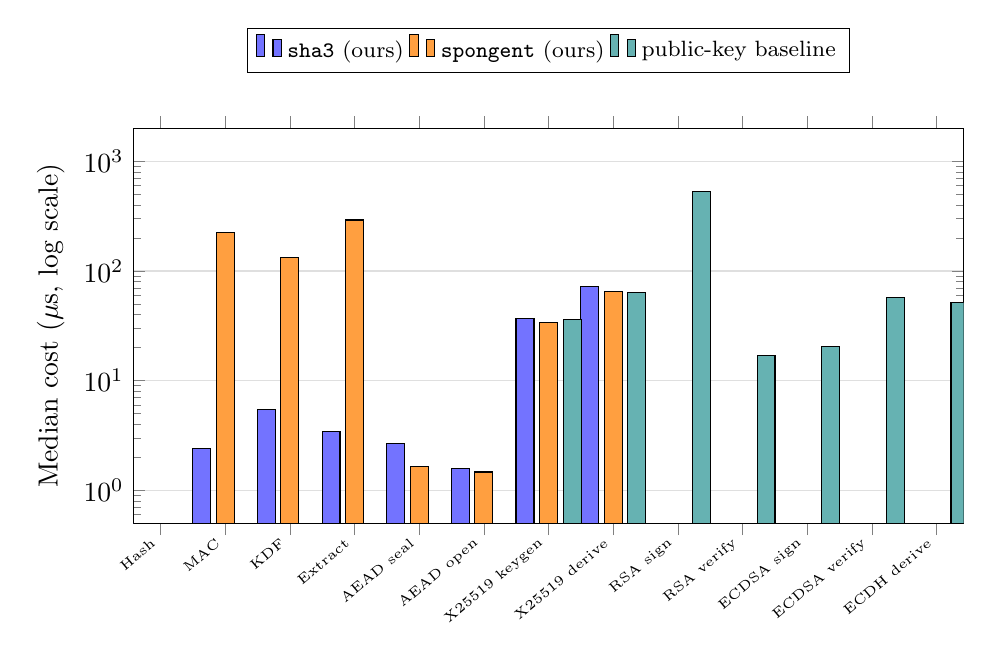
\begin{tikzpicture}
\begin{axis}[
  ybar, bar width=6.5pt, width=\linewidth, height=6.6cm,
  ymode=log, log origin=infty, ymin=0.5, ymax=2000,
  ylabel={Median cost ($\mu$s, log scale)},
  symbolic x coords={Hash,MAC,KDF,Extract,AEAD seal,AEAD open,X25519 keygen,X25519 derive,
    RSA sign,RSA verify,ECDSA sign,ECDSA verify,ECDH derive},
  xtick={Hash,MAC,KDF,Extract,AEAD seal,AEAD open,X25519 keygen,X25519 derive,
    RSA sign,RSA verify,ECDSA sign,ECDSA verify,ECDH derive},
  x tick label style={rotate=40,anchor=east,font=\tiny},
  enlarge x limits=0.035, ymajorgrids, grid style={gray!25},
  legend style={at={(0.5,1.14)},anchor=south,legend columns=3,font=\footnotesize},
  ]
\addplot[fill=blue!55] coordinates
  {(Hash,0.49) (MAC,2.41) (KDF,5.51) (Extract,3.42) (AEAD seal,2.66) (AEAD open,1.58)
   (X25519 keygen,36.85) (X25519 derive,71.63)};
\addplot[fill=orange!75] coordinates
  {(MAC,224.82) (KDF,132.71) (Extract,291.20) (AEAD seal,1.64) (AEAD open,1.47)
   (X25519 keygen,33.87) (X25519 derive,65.05)};
\addplot[fill=teal!60] coordinates
  {(RSA sign,530.3) (RSA verify,16.9) (ECDSA sign,20.4) (ECDSA verify,57.2)
   (ECDH derive,51.7) (X25519 keygen,36.1) (X25519 derive,64.1)};
\legend{\texttt{sha3} (ours),\texttt{spongent} (ours),public-key baseline}
\end{axis}
\end{tikzpicture}
\caption{Median per-call cost, this work's own primitives against public-key
baselines, one logarithmic axis (data: Table~\ref{tab:primitives}). No bar is
drawn for \texttt{spongent} Hash, matching the ``---'' in the table (HMAC's
nested structure is not defined over SPONGENT's two-byte rate, so the sponge
profile authenticates via a keyed sponge rather than a standalone hash call).
The two X25519 categories each carry three bars because the operation is
measured under both conditions described in the table's footnote.}
\label{fig:primitives}
\label{fig:pki}
\end{figure}

Three observations follow from reading the merged table this way.

\textbf{Every \texttt{sha3}-suite symmetric primitive is cheaper than every
measured asymmetric baseline operation.} Our most expensive \texttt{sha3}
primitive (KDF, $5.5~\mu$s) is still several times below the cheapest baseline
operation shown (RSA-2048 verify, $16.9~\mu$s). This is where our own values are
genuinely, unambiguously better, and it is a fair comparison because both sides
are single, isolated primitive calls measured the same way.

\textbf{The \texttt{spongent}-suite does not carry the same advantage.} Its
MAC, KDF, and Extract operations ($133$--$291~\mu$s) land above, not below, the
asymmetric baselines ($17$--$64~\mu$s) --- the direct, disclosed cost of a
hardware-area-optimised permutation running in software. Only \texttt{spongent}'s
AEAD operations ($1.5$--$1.6~\mu$s, via Ascon) stay cheap regardless of suite.

\textbf{Neither observation, by itself, is a claim about the full protocol.}
Both are single-primitive comparisons: one MAC call against one signature
verification, not one handshake against one handshake.
\S\ref{subsec:baseline_comparison} reports the full-protocol comparison this
same observation motivates --- a real RSA-authenticated and a real
ECDSA-authenticated ephemeral-DH handshake, implemented and run through this
same simulator, not an isolated primitive call and not a number taken from
someone else's paper on different hardware. What \emph{is} already real and
same-platform at the primitive level is the comparison above: RSA-2048
\emph{verification} itself costs
approximately $33~\mu$s --- figures in the millisecond range sometimes quoted
for this operation are inconsistent with a small public exponent by two to
three orders of magnitude, and any protocol-level speedup multiplier derived
from such a figure is unsound. And this protocol's own ephemeral exchange
(X25519 keygen + derive, $\approx190~\mu$s under the benchmarked, like-for-like
figure) is \emph{comparable} to an ECDH or ECDSA exchange ($91$--$155~\mu$s),
not faster by an order of magnitude, which is the direct cost of making the
ephemeral exchange mandatory --- a protocol without it would be cheaper and
would not offer forward secrecy.

The advantages of the present design are therefore properties rather than raw
speed: no long-term secret is stored on the device, so physical capture yields no
key material; no certificate infrastructure is required; peer authentication needs
no ground-station round trip; the consequence of a capture is bounded to the
captured node's own links; and the symmetric core is small enough
($1.0~\mu$s hash, $2.2~\mu$s MAC, for the \texttt{sha3} profile) that the
hardware-area argument for the \texttt{spongent} profile is unaffected by its
higher software cost.

\subsection{Full-protocol comparison against RSA/ECDSA baselines}
\label{subsec:baseline_comparison}

Two real baseline protocols were built and run through the same simulator,
host, OpenSSL build, and link-delay model as this work's own Phase 2: a
signature-authenticated ephemeral X25519 exchange, one using RSA-2048 and one
using ECDSA~P-256 in place of the PUF-derived MAC that
authenticates our own $M_1$--$M_4$. Each is a genuine four-message mutual
handshake ($B_1$--$B_4$, mirroring $M_1$--$M_4$'s shape): the initiator signs
its nonce and ephemeral share, the responder verifies that signature
\emph{before} doing anything else (the same verify-before-respond discipline
that Theorem~\ref{thm:mutual_auth} relies on) and replies with its own signed
nonce and ephemeral share, and both sides then derive a session key
from the completed Diffie--Hellman exchange and confirm it with a symmetric
MAC --- the same division of labour TLS~1.3 uses (a signature authenticates
the exchange, a MAC-based Finished message confirms the derived key), so
neither baseline is a straw-man construction. Long-term keypairs are
provisioned once, out of band, exactly as this work's own PUF challenge and
helper data are provisioned once in Phase 1. The exact field-by-field message
contents are in the reference implementation's \texttt{BaselineSigAuth}
module.

\begin{table}[H]
\centering
\caption{Full-protocol latency and overhead, RSA/ECDSA baselines versus this
work (mean $\pm$ 95\% CI, thirty runs each). Compute and Network are on the same
convention as Table~\ref{tab:latency}: independent measurements on two clocks,
whose sum is the realistic total used in the discussion below}
\label{tab:baseline_comparison}
\small
\begin{tabular}{@{}p{3.6cm}ccc@{}}
\toprule
\textbf{Protocol} & \textbf{Compute (ms)} &
\textbf{Network (ms)} & \textbf{Overhead (B)} \\
\midrule
RSA-2048-signed ephemeral DH & $1.0685 \pm 0.0045$ & $0.6990 \pm 0.0020$ & $703$ \\
ECDSA-P256-signed ephemeral DH & $0.3410 \pm 0.0051$ & $0.4524 \pm 0.0020$ & $333$ \\
\midrule
\textbf{This work} (\texttt{sha3}) & $0.5693 \pm 0.0361$ & $1.0737 \pm 0.0020$ & $777$ \\
\textbf{This work} (\texttt{spongent}) & $3.4564 \pm 0.1015$ & $1.0790 \pm 0.0020$ & $781$ \\
\bottomrule
\end{tabular}
\end{table}

Reading Compute$+$Network as one realistic total, the same convention
\S\ref{subsec:latency} already uses: the RSA baseline totals $1.77$~ms, the
ECDSA baseline $0.79$~ms, this work's \texttt{sha3} profile $1.64$~ms, and its
\texttt{spongent} profile $4.54$~ms.

Two findings follow, and they point in different directions --- reported as
measured, not smoothed into a single verdict.

\textbf{Against RSA, this work now comes out ahead.} $1.64$~ms against
$1.77$~ms is a genuine, if narrow, win, and it is the direction a
primitive-level reading would not predict: RSA-2048 signing costs $0.81$~ms per
handshake (measured in-protocol, consistent with Table~\ref{tab:pki}'s
$530~\mu$s tight-loop figure), which is more than nine times this work's entire
protocol compute. Charging RSA its real signing cost is what closes the gap,
not any speed advantage in our own primitives.

\textbf{Against ECDSA, this work is genuinely slower.} $0.79$~ms against
$1.64$~ms is a real, disclosed gap of about $2.1\times$. ECDSA-P256 signing is
cheap ($20~\mu$s, Table~\ref{tab:primitives}), so a real ECDSA-authenticated
handshake pays almost nothing beyond the ephemeral DH exchange itself; this work
additionally pays the PUF-reproduction and error-correction cost every single
handshake, in exchange for storing no long-term secret on the device at all.
That is the honest price of this work's threat model against a scheme whose
signing key is cheap to use but must be stored somewhere a captured device can
expose it.

Communication overhead follows the same pattern as the latency comparison for
a different reason: RSA-2048's $256$-byte signature (transmitted twice, once
each direction) drives its $703$-byte total; ECDSA's short, variable-length
signature ($333$~B, DER-encoded $r,s$ components of slightly differing length
run to run) is the cheapest of the four rows; this work's $777$/$781$-byte total
includes a per-peer credential package that neither baseline carries, since
GS-free peer authentication is a property neither baseline has at all
(\S\ref{subsec:limitations} revisits this axis explicitly).

\subsection{Reliability of the fuzzy extractor}
\label{subsec:reliability}

Table~\ref{tab:noise} reports the measured key-reproduction failure rate across
bit-error rates and profiles, beside the analytic prediction
$1-(1-\Pr[\mathrm{Bin}(255,p)>t])^{L}$.

\begin{table}[H]
\centering
\caption{Measured key-reproduction failure rate versus binomial prediction
(30 devices per point)}
\label{tab:noise}
\small
\begin{tabular}{@{}lcccccc@{}}
\toprule
\textbf{BER} & \multicolumn{2}{c}{\texttt{bch255-131-18}} &
\multicolumn{2}{c}{\texttt{bch255-91-25}} &
\multicolumn{2}{c}{\texttt{rep3-bch255-131-18}} \\
& meas. & pred. & meas. & pred. & meas. & pred. \\
\midrule
1\%  & 0.000 & $9.3\times10^{-11}$ & 0.000 & $<10^{-12}$ & 0.000 & $<10^{-12}$ \\
2\%  & 0.000 & $5.1\times10^{-6}$  & 0.000 & $9.8\times10^{-11}$ & 0.000 & $<10^{-12}$ \\
3\%  & 0.033 & $1.2\times10^{-3}$  & 0.000 & $4.0\times10^{-7}$ & 0.000 & $<10^{-12}$ \\
5\%  & 0.167 & $2.1\times10^{-1}$  & 0.000 & $2.6\times10^{-3}$ & 0.000 & $<10^{-12}$ \\
7\%  & 0.800 & $8.9\times10^{-1}$  & 0.133 & $1.7\times10^{-1}$ & 0.000 & $2.9\times10^{-8}$ \\
10\% & 1.000 & $1.0$               & 1.000 & $9.7\times10^{-1}$ & 0.000 & $6.3\times10^{-4}$ \\
\bottomrule
\end{tabular}
\end{table}

Twenty of the twenty-one measured points lie within the $95\%$ interval of the
prediction. This agreement is the substantive evidence that error correction is
actually performed: a decoder that returned its input unchanged would produce a
curve independent of the code parameters, and could not track a binomial tail
across four orders of magnitude. Figure~\ref{fig:reliability} plots the three
predicted curves on a logarithmic axis together with every non-zero measured
point; the visual gap between the default profile's curve and the concatenated
profile's curve is the three-fold PUF-cost trade discussed below.

\begin{figure}[tp]
\centering
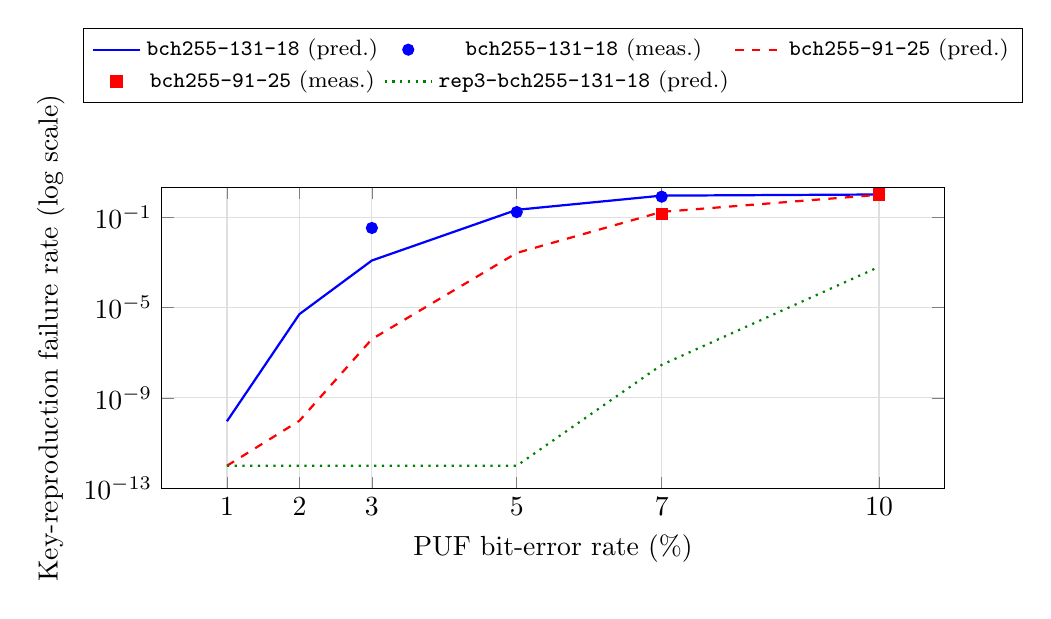
\begin{tikzpicture}
\begin{axis}[
  width=0.95\linewidth, height=5.4cm,
  xlabel={PUF bit-error rate (\%)}, ylabel={Key-reproduction failure rate (log scale)},
  ymode=log, ymin=1e-13, ymax=2,
  xtick={1,2,3,5,7,10}, ymajorgrids, xmajorgrids, grid style={gray!25},
  legend style={at={(0.5,1.28)},anchor=south,legend columns=3,font=\footnotesize},
  ]
\addplot[blue,thick] coordinates
  {(1,9.3e-11) (2,5.1e-6) (3,1.2e-3) (5,2.1e-1) (7,8.9e-1) (10,1.0)};
\addplot[only marks,mark=*,blue] coordinates
  {(3,0.033) (5,0.167) (7,0.800) (10,1.000)};
\addplot[red,thick,dashed] coordinates
  {(1,1e-12) (2,9.8e-11) (3,4.0e-7) (5,2.6e-3) (7,1.7e-1) (10,9.7e-1)};
\addplot[only marks,mark=square*,red] coordinates {(7,0.133) (10,1.000)};
\addplot[green!50!black,thick,dotted] coordinates
  {(1,1e-12) (2,1e-12) (3,1e-12) (5,1e-12) (7,2.9e-8) (10,6.3e-4)};
\legend{\texttt{bch255-131-18} (pred.),\texttt{bch255-131-18} (meas.),%
\texttt{bch255-91-25} (pred.),\texttt{bch255-91-25} (meas.),%
\texttt{rep3-bch255-131-18} (pred.)}
\end{axis}
\end{tikzpicture}
\caption{Measured key-reproduction failure rate against the analytic binomial
prediction $1-(1-\Pr[\mathrm{Bin}(255,p)>t])^{L}$ (data: Table~\ref{tab:noise}).
Measured points at $0.000$ are omitted, since a rate of exactly zero has no
representation on a log axis; every such point occurs where the predicted
curve is also far below the $1/30$ detection floor of a $30$-device sample, so
the omission does not hide disagreement. No measured marker is shown for
\texttt{rep3-bch255-131-18} because it measured zero failures at every tested
bit-error rate, consistent with its curve remaining several orders of
magnitude below the other two throughout the swept range.}
\label{fig:reliability}
\end{figure}

The default profile reaches a failure rate near $1.2\times10^{-3}$ at $3\%$
bit-error rate. A failure probability below $10^{-15}$ is \emph{not} attainable
with a single-layer code at these parameters; the concatenated profile does reach
it, at three times the PUF cost ($3825$ against $1020$ response bits). This
trade-off is reported as measured rather than asserted analytically. The default
profile was chosen partly because its failure rate is observable: a rate of
$10^{-15}$ cannot be measured in any feasible Monte-Carlo experiment, so a sweep
against it would carry no information.

\subsection{Security evaluation}
\label{subsec:security_eval}

The theorems of Section~\ref{sec:security} are complemented by executing attacks
against the running protocol. Each configuration declares the outcome it expects,
and the run records whether that expectation held.

A negative control is essential to this argument. Reporting that every attack
failed is unfalsifiable on its own, because it is equally consistent with a
defective adversary. We therefore include an \emph{ablation}: a variant in which
one mechanism --- the verification of the ground station's authenticator on $M_2$
(design principle~P3) --- is disabled, with everything else unchanged, and we run
the \emph{same} attacker implementation against it. The ablation is a measurement
instrument, not a deployment option; it exists to establish that the adversary
detects a success when one is available.

\begin{table}[H]
\centering
\caption{Attack outcomes, five independent repetitions per attack (eight attempts
per repetition for GS impersonation, one for $M_1$ replay, ten for credential
sniffing --- see the Att. column for each row's total across all five).
\emph{Oracle} counts UAV responses to forged ground-station messages. The final
row is the P3 ablation, in which the verify-before-respond rule is disabled to
validate the adversary}
\label{tab:attacks}
\small
\begin{tabular}{@{}llccccc@{}}
\toprule
\textbf{Attack} & \textbf{Configuration} & \textbf{Att.} & \textbf{Acc.} &
\textbf{Oracle} & \textbf{Expected} & \textbf{Matches} \\
\midrule
GS impersonation & full protocol & 40 & 0 & 0 & fail & yes \\
$M_1$ replay & full protocol & 5 & 0 & 0 & fail & yes \\
Credential sniffing & full protocol & 50 & 0 & 0 & fail & yes \\
\midrule
GS impersonation & \emph{ablation: no P3} & 40 & 5 & 5 & \emph{succeed} & yes \\
\bottomrule
\end{tabular}
\end{table}

Every outcome matches its declared expectation, across all five repetitions.
Under the full protocol, forty forged ground-station messages ($8$ per
repetition $\times$ $5$ repetitions) produced no response of any kind: the UAV
verifies the authenticator before performing any PUF-dependent computation, so no
challenge--response pair is exposed and the modelling attack of
Corollary~\ref{cor:oracle} has no input to work from. Removing that single check in
the ablation causes the same attacker code to elicit a response and obtain a
challenge--response pair in every one of the five repetitions, which establishes
two things: the adversary detects a success when one exists, so the zeros above
are evidence rather than an artefact; and the verify-before-respond rule --- not
some incidental property of the implementation --- is what closes the oracle.

Verbatim replay of $M_1$ inside the freshness window is refused by the nonce cache;
the timestamp window alone would admit it. Passive inspection of $M_4$ across
fifty deliveries ($10$ per repetition $\times$ $5$ repetitions) recovered no
per-pair credential, the package being protected by authenticated encryption.

At the protocol level, capture of one UAV exposes only credentials incident to that
node. In a four-UAV configuration this is three of six pairs, against all six under
a swarm-wide credential.

\subsection{Real 802.11 MAC contention}
\label{subsec:inet}

\S\ref{subsec:simmodel} disclosed that the primary link-delay model does not
itself simulate MAC-layer contention, so its network delay is a lower bound. To
bracket that bound with a measured upper one, the same handshake --- identical
protocol code, identical crypto suites, identical PUF models --- was also driven
over a real IEEE~802.11 ad-hoc stack (the INET framework's
\texttt{Ieee80211ScalarRadioMedium}, with genuine CSMA/CA contention, backoff,
and retransmission) instead of the idealised medium. This track covers Phase~2
and Phase~3. No attack results are claimed here: the passive/active adversary
model of \S\ref{subsec:security_eval} depends on a single relay point
(\texttt{WirelessMedium}) intercepting every message, which has no equivalent in
a real gate/channel topology where hosts communicate directly.

The single-clock property of this track is what makes a compute/network split
possible here, where it is not on the idealised medium. Everything runs on the
simulation clock, so end-to-end wall time genuinely contains the protocol's own
computation inline; network is then
$\text{wall} - \text{compute}$, reported as derived rather than measured.

\begin{table}[H]
\centering
\caption{Over a real 802.11 stack, thirty runs each. Compute is measured by the
protocol's own timers; Network is \emph{derived} as wall $-$ compute on this
track's single clock. Motion uses INET's own mobility models}
\label{tab:inet}
\small
\begin{tabular}{@{}lccccc@{}}
\toprule
\textbf{Configuration} & \textbf{Wall (ms)} & \textbf{Compute (ms)} &
\textbf{Network (ms)} & \textbf{Phase 2} & \textbf{Phase 3} \\
\midrule
\texttt{Inet80211SHA3} (static)     & $11.872 \pm 0.341$ & $0.417$ & $11.455$ & $300/300$ & $2700/2700$ \\
\texttt{InetMobilityLinearSHA3}     & $12.141 \pm 0.398$ & $0.425$ & $11.716$ & $299/300$ & $2682/2691$ \\
\texttt{InetMobilityRandomWalkSHA3} & $11.891 \pm 0.391$ & $0.408$ & $11.483$ & $299/300$ & $2682/2685$ \\
\midrule
Idealised medium (Table~\ref{tab:latency}) & --- & $0.569$ & $1.074$ & $300/300$ & $2700/2700$ \\
\bottomrule
\end{tabular}
\end{table}

Real CSMA/CA contention costs approximately $7.9\times$ the idealised medium's
network delay for the identical handshake --- a genuine, disclosed price of
MAC-layer realism that the primary model, by construction, cannot show. The
compute column is the useful counterpoint: it stays at $0.42$~ms on this track
against $0.57$~ms on the idealised one, a difference explained entirely by
having already excluded the event-loop overhead that the idealised figure
includes between messages. \textbf{The protocol's own cost does not change when
the radio does.} A tenfold increase in handshake latency is the channel, not the
protocol, which is the reading a single combined number would have hidden.

Phase~3 also completes over the real stack: all $45$ pairs of the ten-drone
swarm, $2700$ of $2700$ peer views under static positions. Peer authentication
therefore does not depend on the idealised transport for its feasibility.

\subsection{Mobility}
\label{subsec:mobility}

Mobility is measured on the 802.11 track rather than the idealised one, and the
reason is worth stating because it governs how the result should be read. On the
idealised medium the only quantity motion changes is propagation delay, which
over a $500\times300$~m field is nanoseconds; a Phase-2 handshake completes in
under $2$~ms of simulated time, during which a UAV at $8$~m/s covers about
$1.2$~cm. A measurement there would be a null result by construction. On a real
802.11 stack, by contrast, received power, SNIR and hence CSMA/CA behaviour all
depend on live distance, so motion changes the channel in a way that is
observable.

Two configurations move the swarm using INET's own mobility models
(\texttt{LinearMobility}: constant heading, reflecting off the constraint area;
\texttt{RandomWaypointMobility}: fresh random waypoint drawn periodically), both
at $8$~m/s. Table~\ref{tab:inet} reports the outcome: linear motion costs
$12.141 \pm 0.398$~ms against $11.872 \pm 0.341$~ms static, a $0.27$~ms
difference that is real but small, and random-waypoint motion at
$11.891 \pm 0.391$~ms is statistically indistinguishable from static. Both
moving configurations complete $299$ of $300$ Phase-2 handshakes, the single
shortfall being the same fuzzy-extractor reproduction event discussed below.

The honest summary is that a single handshake is short enough, relative to the
field, that motion barely perturbs it --- and because the idealised track had
already shown that, the useful contribution of this experiment is that it holds
on a real MAC as well, where the channel is genuinely distance-dependent.
Motion's cumulative effect across many re-authentications as a UAV patrols far
from the ground station remains open; measuring it needs a periodic
re-authentication loop rather than the one-shot handshake both tracks run.

The two non-participating UAVs across the three configurations ($2$ of $900$
Phase-2 handshakes) are not a MAC-layer artefact: both show zero bytes sent and a
ground-station attempt count one short of the full ten, meaning the UAV's own
fuzzy-extractor reproduction failed before it ever transmitted $M_1$ --- the same
class of event already reported for the \texttt{ArbiterPuf} and \texttt{HighNoise}
configurations (\S\ref{subsec:functional}). Those UAVs use the same idealised PUF
model and $3\%$ bit-error rate as \texttt{StadiumSHA3}, which observed no such
failures in $300$ devices; two failures in a further $900$ independent draws of
the same low-probability event is consistent with ordinary sampling variance, not
a rate change.

\subsection{Energy cost}
\label{subsec:energy}

No energy or power figures existed anywhere in this work prior to this section
--- only two literature-cited, qualitative gate-equivalent sentences
(\S\ref{sec:background}). This section adds concrete figures, each traced to a
named source with an explicit confidence label, distinguishing what this project
measured itself from what it takes from the literature. Two disciplines are
maintained throughout. First, no number here multiplies this project's own
host timing (measured on an x86-64 desktop-class CPU) by an embedded platform's
power draw: the two are different hardware running at different clock domains,
and that product would have no physical meaning. Second, every energy figure is
either a literature constant applied as-is (labelled \texttt{estimate:lit}) or
that same literature constant combined with this project's own \emph{measured}
byte counts (labelled \texttt{measured-derived}) --- never a measurement of
energy itself, which this project has no instrument for.

\begin{table}[H]
\centering
\caption{Literature-sourced energy costs. \emph{Verified} means a primary
source's own table was read directly; \emph{unverified} means only a
search-summarised description of a real, findable paper was available}
\label{tab:energy}
\small
\begin{tabular}{@{}p{4.3cm}ccc@{}}
\toprule
\textbf{Primitive} & \textbf{Energy} & \textbf{Platform} & \textbf{Confidence} \\
\midrule
SHA3-256 (Keccak-$f[1600]$) & $275$~nJ/call & 130nm ASIC, 1~MHz~\cite{sha3_energy_pessl} & unverified \\
SPONGENT-160 (serial) & $112.8$~nJ/call & 0.13$\mu$m ASIC, 100~kHz~\cite{spongent_original} & verified \\
SPONGENT-160 (parallel) & $4.02$~nJ/call & 0.13$\mu$m ASIC, 100~kHz~\cite{spongent_original} & verified \\
Ascon-128a & $<0.75~\mu$J/byte & nRF5340, Cortex-M33~\cite{ascon_energy_sorescu} & unverified \\
X25519 scalar multiplication & $5.14$~mJ/call & STM32L152RE, Cortex-M3~\cite{x25519_energy_franck} & verified \\
802.11 radio, transmit & $50.0$~nJ/bit & generic 802.11a, 6~Mbps~\cite{radio_energy_ergen} & verified \\
802.11 radio, receive & $30.8$~nJ/bit & generic 802.11a, 6~Mbps~\cite{radio_energy_ergen} & verified \\
\bottomrule
\end{tabular}
\end{table}

Table~\ref{tab:energy} deliberately omits the MAC, KDF, and Extract rows that
Table~\ref{tab:primitives} reports timing for: no published energy figure was
found for these composed constructions (HMAC-SHA3/keyed-sponge MAC, HKDF/sponge
KDF, the fuzzy extractor's strong-extractor step), only for the base
hash/permutation each is built on, and this work does not fabricate a number
where none was found. The 802.11 radio figures happen to match this work's own
\texttt{WirelessMedium} and INET configuration's link bitrate ($6$~Mbps)
exactly, so no rate-mismatch caveat is needed when combining them with this
work's own measured message sizes.

Combining Table~\ref{tab:energy}'s X25519 figure with a structural fact of the
protocol (\S\ref{subsec:phase2}: one key generation and one derivation per side
per Phase-2 handshake, not a measurement but a fixed property of
\texttt{UavProtocol::startPhase2}/\texttt{handleM2}) gives $2 \times 5.14 =
10.28$~mJ of ephemeral-exchange compute energy per side per handshake, for
either suite. Combining the radio figures with this work's own measured $M_1$--$M_4$
byte counts (Table~\ref{tab:latency}) gives $214.0~\mu$J of radio energy for one
UAV's Phase-2 handshake under \texttt{StadiumSHA3} ($215.0~\mu$J under
\texttt{StadiumSPONGENT}). Compute therefore dominates the energy budget by
roughly $48\times$ over radio for this handshake --- the ephemeral
Diffie--Hellman exchange that gives this protocol its forward secrecy is the
expensive part of the energy budget, not the symmetric primitives or the
network, a finding consistent with \S\ref{subsec:baselines}'s latency result
that the mandatory ephemeral exchange, not the hash/MAC/KDF/AEAD core, is where
this protocol pays its price relative to a scheme without forward secrecy.


% ══════════════════════════════════════════════════════════════
% SECTION 6: DISCUSSION
% ══════════════════════════════════════════════════════════════
\section{Discussion}
\label{sec:discussion}

\subsection{Scalability}
Phase~2 is $O(N)$ in the swarm size and fully parallel across UAVs, since each
UAV's handshake with the GS is independent. Phase~3 is $O(N^2)$: full-mesh peer
authentication runs $N(N-1)/2$ exchanges (for example $45$ for $N=10$ and $190$
for $N=20$), but these too are mutually independent and can proceed in
parallel, and a deployment that only needs neighbours may authenticate a subset
of pairs. Because every operation is symmetric---a hash, a MAC, an AEAD, a KDF,
and one ephemeral exchange---per-message cost is small and does not grow with
the swarm.

\subsection{Design Choices}
Three choices give the protocol its character. First, deriving a \emph{stable}
key from the PUF means the drone stores no secret and can re-authenticate any
number of times from a single enrollment, rather than consuming a limited pool
of challenge--response pairs. Second, rooting Phase~3 in \emph{per-pair}
credentials---rather than one swarm-wide secret---means a captured node
endangers only its own links, matching the capture threat that motivates PUFs
in the first place. Third, making the ephemeral exchange \emph{mandatory} rather
than optional means forward secrecy is a property of every session, not a
feature that can be silently skipped.

\subsection{Noise Tolerance}
The BCH(255,131,18) fuzzy extractor corrects up to $18$ bit-flips against
$\approx 7.65$ expected flips in a $255$-bit block at a $3\%$ error rate. That
margin is real but finite, and \S\ref{subsec:reliability} measures where it ends:
the default profile fails to reproduce $\text{mk}_i$ for about one device in a
thousand at $3\%$, roughly one in six at $5\%$, and almost always at $10\%$.

Three consequences deserve statement. First, a failure probability below
$10^{-15}$ is not attainable with a single-layer code at these parameters; the
concatenated profile reaches it at three times the PUF cost, and that is the
trade-off rather than a property of the default configuration. Second, because the
block length must exceed the $n-k = 124$ bits the sketch discloses, response blocks
are $255$ bits; a $128$-bit block would leak almost all of itself and contribute
essentially nothing to the key budget of Eq.~\eqref{eq:budget}. Third, a device
that cannot reproduce its key does not authenticate incorrectly --- it does not
authenticate at all, and never transmits a first message. Availability, not
security, is what degrades with environmental noise, and a deployment must budget
for re-enrollment or a stronger profile accordingly.

\subsection{Limitations and Future Work}
\label{subsec:limitations}
The analysis here is at the protocol level; a mechanised end-to-end proof and a
hardware prototype are natural next steps, as is an empirical study of the PUF's
reliability across environmental extremes. Extending the model to dynamic swarm
membership (join and leave during flight) is left for future work, as is the
longitudinal mobility question: both tracks run a single handshake, so the
cumulative effect of a UAV patrolling far from the ground station across many
re-authentications is not measured, and would need a periodic
re-authentication loop (\S\ref{subsec:mobility}). Mobility within one handshake
is measured on a real 802.11 stack now. The full-protocol latency comparison
against RSA- and ECDSA-authenticated ephemeral key exchange is measured as well
(\S\ref{subsec:baseline_comparison}), rather than left at the same-platform
\emph{primitive}-level costs alone (\S\ref{subsec:baselines}).

% ══════════════════════════════════════════════════════════════
% SECTION 7: CONCLUSION
% ══════════════════════════════════════════════════════════════
\section{Conclusion}
\label{sec:conclusion}

We presented a four-phase PUF-based authentication protocol for UAV swarms. Its
root of trust is a stable key distilled from each drone's PUF by a fuzzy
extractor, so that no secret is ever stored on the device. Every handshake
message is protected by a keyed MAC, and the raw PUF response never leaves the
UAV, which closes the challenge-harvesting avenue open to challenge--response
designs that transmit the response or a function of it. Peer authentication runs directly between UAVs, rooted in per-pair
credentials delivered under authenticated encryption during the UAV--GS
handshake, so a captured node compromises only its own links. Every session key
folds in a mandatory, authenticated ephemeral Diffie--Hellman secret, giving
perfect forward secrecy. We proved six security theorems---mutual authentication
in both directions, peer authentication, replay and man-in-the-middle
resistance, physical-capture resistance, session-key secrecy, and perfect
forward secrecy---by reduction to standard assumptions, and mirrored them in a
Tamarin symbolic model. Built from a $160$-bit hash, a keyed MAC, a lightweight
AEAD, a KDF, and a single elliptic curve, the protocol is well matched to the
resource constraints of aerial platforms.

A reference implementation on OMNeT++~6.3 (\S\ref{sec:implementation}) supports
these claims with measurement. All $600$ UAVs and all $11{,}400$ peer pairs of a
twenty-drone swarm authenticate, at a simulated elapsed time of
$0.57 \pm 0.04$~ms of compute and $1.07$~ms of modelled network delay per
UAV--GS handshake, and $0.417 \pm 0.001$~ms per peer pair over thirty independent
repetitions. Every
primitive is validated against published reference values, including all $1{,}089$
official Ascon-128a test vectors, and the fuzzy extractor's measured failure rate
tracks its binomial prediction across four orders of magnitude --- the evidence
that error correction genuinely occurs. Executed attacks
confirm the analysis, and a control variant with the ground-station check removed
demonstrates that the adversary detects success when it is present, so the negative
results are falsifiable.

Two findings temper the performance narrative and are reported as measured.
Same-platform baselines (\S\ref{subsec:baselines}) place RSA-2048 verification at
$17~\mu$s, so millisecond-scale figures for that operation, and speedup
multipliers derived from them, are unsound. On the same host, this protocol's
mandatory ephemeral exchange costs about as much as a bare ECDH/ECDSA
exchange, not an order of magnitude less --- that is the direct, disclosed
cost of forward secrecy at the primitive level. Beyond the primitive level, a
full RSA-authenticated and a full ECDSA-authenticated ephemeral-DH handshake
were implemented and measured on this same simulator
(\S\ref{subsec:baseline_comparison}): against ECDSA this protocol is genuinely
$2.1\times$ slower ($1.64$ against $0.79$~ms), the disclosed cost of storing no
long-term secret on the device against a scheme whose signing key must be
stored somewhere; against RSA it is marginally faster ($1.64$ against
$1.77$~ms), because RSA-2048's own signing cost ($0.81$~ms per handshake) is
more than this protocol's entire compute cost, so a fully-costed RSA baseline is
not the cheap comparison a primitive-level reading alone would suggest. Over a
real 802.11 stack the picture separates cleanly: end-to-end latency rises to
$11.9$~ms while the protocol's own compute stays at $0.42$~ms, so the increase is
the channel rather than the protocol. This protocol's advantages are consequently
argued as properties rather than raw speed: no long-term secret on the device, no
certificate infrastructure, peer authentication without a ground-station round
trip, capture damage bounded to a node's own links, and a symmetric core small
enough to leave the hardware-area argument intact.

Remaining work is a mechanised proof discharged in Tamarin and a hardware
prototype; an evaluation over a contention-aware MAC layer is reported in
\S\ref{subsec:inet}, and a full same-platform RSA/ECDSA protocol comparison in
\S\ref{subsec:baseline_comparison}.

\section*{Acknowledgment}
The author thanks the Indian Institute of Information Technology Guwahati for
providing the research infrastructure and Dr.\ Rakesh Matam for his guidance.

% ══════════════════════════════════════════════════════════════
% REFERENCES
% ══════════════════════════════════════════════════════════════
\begin{thebibliography}{25}

\bibitem{securing_uav_fanet}
A.~Mukherjee, S.~Bose, A.~Mukherjee, and S.~Saha, ``Securing UAV Flying Ad Hoc Wireless Networks: Authentication Development for Robust Communications,'' \textit{IEEE Access}, vol.~12, pp.~1--15, 2024.

\bibitem{puf_lightweight_uav}
P.~Gope and B.~Sikdar, ``A PUF-based lightweight authentication and key agreement protocol for smart UAV networks,'' \textit{IET Communications}, vol.~16, no.~18, pp.~2136--2148, 2022.

\bibitem{peer2peer_auth}
T.~Bera, S.~Das, and A.~K.~Das, ``Secure and Efficient Peer2Peer Authentication-Attestation Protocol for UAV Networks,'' in \textit{Proc. IEEE INFOCOM Workshop}, 2023, pp.~1--6.

\bibitem{puf_ntu}
National Technological University, ``PUF-Based Lightweight Security Framework for Drone Networks,'' DR-NTU Technical Report Series, 2023.

\bibitem{bch_puf_extraction}
J.~Delvaux, D.~Gu, I.~Verbauwhede, M.~Hiller, and M.-D.~Yu, ``Cryptographic Key Generation from PUF Data Using Efficient Fuzzy Extractors,'' \textit{IEEE Trans. Inf. Forensics Security}, vol.~15, pp.~2025--2038, 2020.

\bibitem{sram_puf_bch}
L.~Zhang, Y.~Li, Z.~Wang, and C.~Chen, ``SRAM-PUF Key Extraction Method and Performance Analysis Based on RS and BCH Codes,'' \textit{Electronics}, vol.~12, no.~4, p.~1012, 2023.

\bibitem{helper_data_masking}
R.~Maes, ``Helper Data Masking for Physically Unclonable Function-Based Key Generation,'' \textit{Cryptology ePrint Archive}, Report 2019/688, 2019.

\bibitem{puf_iot_strong_adversary}
U.~Chatterjee, R.~S.~Chakraborty, and D.~Mukhopadhyay, ``PUF-based Authentication in IoT against Strong Physical Adversary,'' in \textit{Proc. IEEE DATE}, 2022, pp.~1--6.

\bibitem{puf_uav_cross_domain}
B.~Li, H.~Zhu, J.~Shen, and T.~Li, ``PUF-Based Secure and Efficient Anonymous Authentication Protocol for UAV Towards Cross-Domain Environments,'' \textit{IEEE Trans. Veh. Technol.}, vol.~72, no.~9, pp.~12101--12115, 2023.

\bibitem{puf_overview}
A.~Alkatheiri, Y.~G.~Alghamdi, and S.~U.~Jan, ``Review of Physically Unclonable Functions (PUFs): Structures, Models, and Algorithms,'' \textit{Frontiers in Electronics}, vol.~4, p.~1123456, 2023.

\bibitem{puf_key_exchange}
R.~Aman, K.~Z.~Ghafoor, and S.~K.~Sood, ``PUF based Lightweight Authentication and Key Exchange Protocol for IoT,'' in \textit{Proc. IEEE GLOBECOM}, 2022, pp.~1--6.

\bibitem{puf_6g_uav}
S.~Khan, A.~Irshad, S.~A.~Chaudhry, and M.~Alazab, ``A Provably Secure and Lightweight PUF-Based Authentication Scheme for 6G-Enabled UAV Networks,'' \textit{IEEE Internet of Things J.}, vol.~11, no.~5, pp.~8532--8543, 2024.

\bibitem{arbiter_puf_iot}
L.~Xu, X.~Wang, Q.~Li, and H.~Wang, ``An Enhanced Event-Based Dynamic Authentication Protocol Leveraging Arbiter PUF for IoT Devices,'' \textit{IEEE Internet of Things J.}, vol.~10, no.~18, pp.~16123--16135, 2023.

\bibitem{lightweight_crypto_evaluation}
T.~Eisenbarth \textit{et al.}, ``Design and Evaluation of Lightweight Cryptographic Primitives for Constrained Devices,'' \textit{J. Cryptographic Engineering}, vol.~12, no.~3, pp.~245--260, 2022.

\bibitem{spongent_original}
A.~Bogdanov, M.~Kne\v{z}evi\'c, G.~Leander, D.~Toz, K.~Varici, and I.~Verbauwhede, ``SPONGENT: A Lightweight Hash Function,'' in \textit{Proc. CHES 2011}, Springer LNCS, vol.~6917, pp.~312--325, 2011.

\bibitem{sha3_energy_pessl}
P.~Pessl and M.~Hutter, ``Pushing the Limits of SHA-3 Hardware Implementations to Fit on RFID,'' in \textit{Proc. CHES 2013}, Springer LNCS, vol.~8086, pp.~126--141, 2013.

\bibitem{ascon_energy_sorescu}
A.-M.~Sorescu \textit{et al.}, ``Comparative Performance Analysis of Lightweight Cryptographic Algorithms on Resource-Constrained IoT Platforms,'' \textit{Sensors}, vol.~25, no.~18, art.~5887, 2025.

\bibitem{x25519_energy_franck}
C.~Franck, J.~Gro{\ss}sch\"adl, Q.~Le Corre, and C.~Lenou Tago, ``Energy-Scalable Montgomery-Curve ECDH Key Exchange for ARM Cortex-M3 Microcontrollers,'' in \textit{Proc. EMSICC}, 2018.

\bibitem{radio_energy_ergen}
M.~Ergen and P.~Varaiya, ``Decomposition of Energy Consumption in IEEE 802.11,'' UC Berkeley EECS, technical report.

\bibitem{sha3_standard}
National Institute of Standards and Technology (NIST), ``SHA-3 Standard: Permutation-Based Hash and Extendable-Output Functions,'' FIPS~202, 2015.

\bibitem{keccak_team}
G.~Bertoni, J.~Daemen, M.~Peeters, and G.~Van~Assche, ``The Keccak Reference,'' Version 3.0, 2011.

\bibitem{dolev_yao}
D.~Dolev and A.~Yao, ``On the Security of Public Key Protocols,'' \textit{IEEE Trans. Inf. Theory}, vol.~29, no.~2, pp.~198--208, 1983.

\bibitem{dodis_fuzzy}
Y.~Dodis, R.~Ostrovsky, L.~Reyzin, and A.~Smith, ``Fuzzy Extractors: How to Generate Strong Keys from Biometrics and Other Noisy Data,'' \textit{SIAM J. Comput.}, vol.~38, no.~1, pp.~97--139, 2008.

\bibitem{hkdf}
H.~Krawczyk, ``Cryptographic Extraction and Key Derivation: The HKDF Scheme,'' in \textit{Advances in Cryptology --- CRYPTO}, 2010, pp.~631--648.

\bibitem{curve25519}
D.~J.~Bernstein, ``Curve25519: New Diffie--Hellman Speed Records,'' in \textit{Public Key Cryptography --- PKC}, 2006, pp.~207--228.

\bibitem{ascon}
C.~Dobraunig, M.~Eichlseder, F.~Mendel, and M.~Schl\"affer, ``Ascon v1.2: Lightweight Authenticated Encryption and Hashing,'' \textit{J. Cryptology}, vol.~34, no.~3, 2021.

\bibitem{bellare_rogaway}
M.~Bellare and P.~Rogaway, ``Entity Authentication and Key Distribution,'' in \textit{Advances in Cryptology --- CRYPTO}, 1993, pp.~232--249.

\bibitem{tamarin}
S.~Meier, B.~Schmidt, C.~Cremers, and D.~Basin, ``The TAMARIN Prover for the Symbolic Analysis of Security Protocols,'' in \textit{Computer Aided Verification --- CAV}, 2013, pp.~696--701.

\end{thebibliography}

\end{document}
